
\chapter{Architektura}
\label{sec:Architektura}

\section{Inkubator}

\subsection{Konstrukcja}
Większość współczesnych inkubatorów ma konstrukcję zewnętrzną polimerową
(np.~z~poliuretanu) albo zbudowaną z~kątowników aluminiowych i~sklejki.
Konstrukcje te są produkowane seryjnie w~profesjonalnych zakładach.
Najczęściej obudowy polimerowe są odlewami. Koszt wykonania takiej formy przekracza
nawet 10~tysięcy~zł. 

Konstrukcję zewnętrzną inkubatora wykonano z~płyty wiórowej, ponieważ jest ona
łatwiejsza w~obróbce niż polimery, natomiast obudowa aluminiowo-sklejkowa jest
droższa i~jej wykonanie jest bardziej czasochłonne (porównywalna konstrukcja
musiałaby się składać z~23~elementów) niż wykonanie obudowy z~płyty wiórowej (7~elementów).
Największą wadą płyty wiórowej jest jej niska odporność na wilgoć. Rozwiązano
ten problem zapewniając szczelność na poziomie polietylenowej konstrukcji
wewnętrznej, która została profesjonalnie zespawana, więc jest w~100\%
hermetyczna. 

Konstrukcja zewnętrzna jest podzielona na dwie części -- inkubacyjną i~techniczną.
W~części inkubacyjnej o~rozmiarze 60~cm~x~50~cm~x~50~cm mieści się
komora inkubacyjna oraz 10-milimetrowa warstwa izolacji styropianowej.
Część techniczna ma rozmiar 20~cm~x~50~cm~x~50~cm i~zawiera przestrzeń na wymiennik
ciepła, silnik oraz system sterowania. 

Konstrukcja wewnętrzna (,,komora inkubacyjna'') jest wykonana z~polietylenu --
bardzo gładkiego i~śliskiego materiału, ułatwiającego mycie i~sterylizację -- to
bardzo istotne dla pracowników ogrodu zoologicznego. Co więcej, polietylen posiada atest na
kontakt z~żywnością, więc jest niegroźny dla piskląt. Komora inkubacyjna
została połączona z~konstrukcją zewnętrzną, aby usztywnić całą konstrukcję
inkubatora. Komora ta wyposażona jest w~dwie ramki o~rozmiarze
43~cm~x~40~cm~x~4~cm, które mogą utrzymać około 50 jaj kurzych. Jej rozmar wynosi 58~cm~x~48~cm~x~48~cm, co zapewnia ramkom odpowiednią przestrzeń, aby
jaja o~wymaganym rozmiarze mogły się obrócić.

Aby odizolować komorę inkubacyjną od konstrukcji zewnętrznej oraz wymiennik
ciepła od reszty części technicznej użyto styropianu. Może on wytrzymać temperaturę rzędu 80\st{} (wymiennik ciepła może
się rozgrzać nawet do 60\st).

% obrazek inkubatora 

\subsection{Projekt mechaniczny}
Obecnie stosuje się dwie technologie obracania jaj:

\begin{itemize}
\item rotacja częściowa - jaja są wkładane pionowo w~specjalne ramki, które utrzymują je
wychylając się pod pewnym kątem. To rozwiązanie jest najczęściej używane
w~inkubatorach jaj strusich (ze względu na ich rozmiar oraz na cechy gatunku)
oraz w~inkubatorach drobiu na skalę przemysłową (ze względu na małą utratę
miejsca w~inkubatorze);

\item rełna rotacja - jaja są wkładane poziomo na rolki obracające się o~180\st{} w~przeciwnych
kierunkach. To~rozwiązanie jest trudniejsze w~konstrukcji oraz wymaga
dodatkowego miejsca, gdyż w~większości implementacji tego rozwiązania rolki z~jajami
przemieszczają się w~poziomie. Z~drugiej strony uważa się, że~to rozwiązanie daje większą
szansę na sukces podczas inkubacji.
\end{itemize}
W~Inkubatorze wybrano mechanizm pełnej rotacji, ze względu na to, że~celem projektu jest
maksymalizacja prawdopodobieństwa sukcesu podczas inkubacji -- każde pisklę może
się okazać bezcenne.
 
Główną częścią systemu rotacyjnego jest silnik elektryczny z~mechanizmem
samopowrotowym (w~momencie, gdy napotka opór zmienia kierunek ruchu).
Silnik napędza śrubę trapezową o~skoku 4~mm z~trzema nakrętkami -- jedną ,,napędową''
oraz dwoma ,,blokującymi''. Nakrętka ,,napędowa'' połączona jest
z~ramkami za pomocą płaskownika aluminiowego natomiast nakrętki ,,blokujące'' 
nakręcone są w~miejscu gdzie mechanizm rotacji ma zawrócić (połowa obwodu
inkubowanych jaj). W~momencie gdy nakrętka napędowa połączy się z~blokującymi,
silnik odbija i~śruba zaczyna się kręcić w~przeciwną stronę.

Do~inkubatora załączonych jest dwadzieścia rolek, które można zamocować w~ramkach
idealnie dopasowując odległość między nimi do rozmiarów inkubowanych jaj. Model
ramek z~rolkami przedstawiony jest na rysunku~\ref{rys:rolki}.

\begin{figure}[t] 
	\centering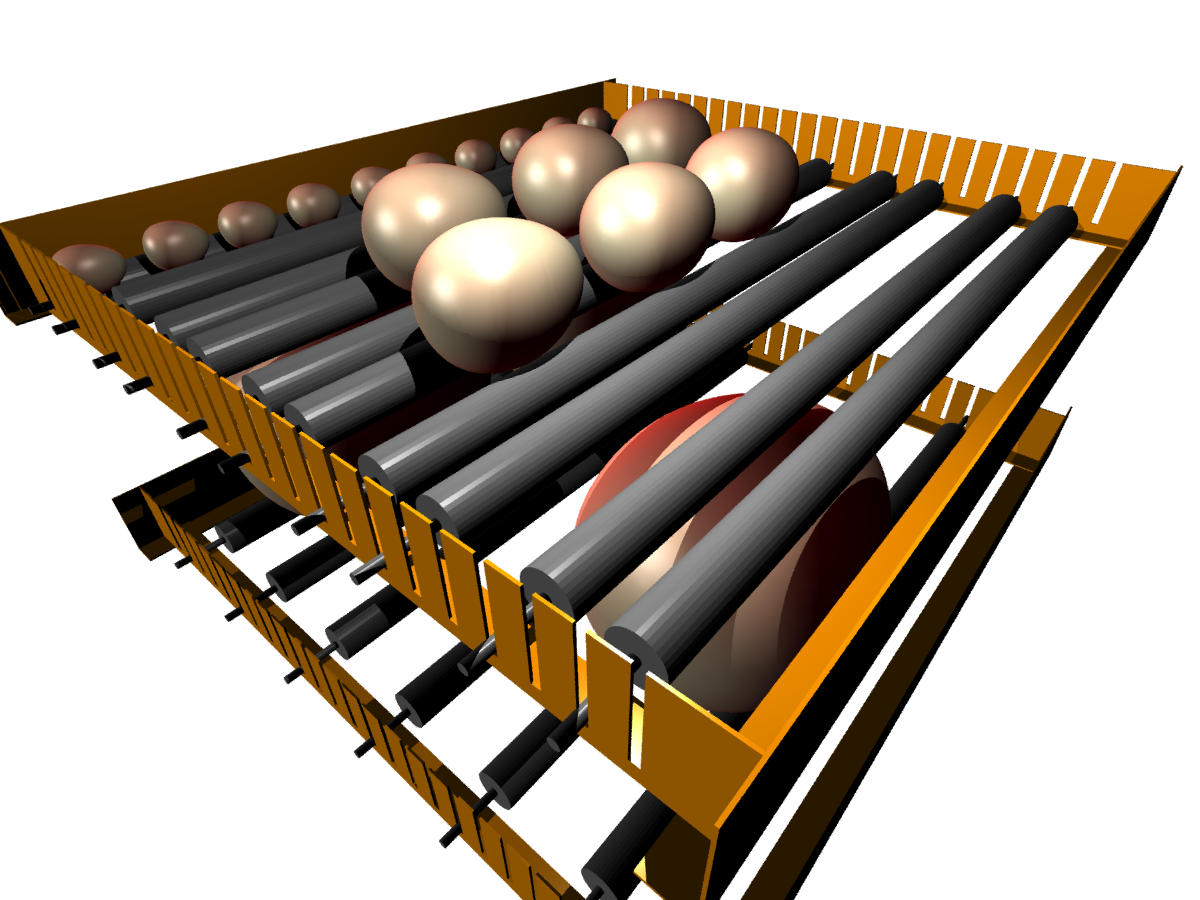
\includegraphics[width=\textwidth]{figures/rolki}
	\caption{Model ramek z~rolkami}\label{rys:rolki}
\end{figure}

\subsection{Wymiennik ciepła}
Sterowanie temperaturą z~dokładnością dochodzącą do $0,1$\st{} jest bardzo
trudnym zadaniem, dlatego potrzebny jest dobry system urządzeń wykonawczych.
Obecnie stosuje się trzy typy rozwiązań:
\begin{itemize}
	\item bezpośrednie podgrzewanie powietrza przez grzałki zainstalowane w~podłodze, 
	\item płaszcz wodny -- podgrzewanie wody otaczającej komorę inkubacyjną --
		rozwiązanie bardzo trudne w~wykonaniu (2 szczelne warstwy, wymuszanie ruchu
		wody na tym obszarze), lecz daje się dość dobrze nim sterować,
	\item podgrzewanie powietrza poza komorą inkubacyjną -- dość łatwe w~wykonaniu
		i~sterowaniu; trudność konstrukcyjna polega na odpowiednim pobraniu
		powietrza z~komory inkubacyjnej i~wprowadzeniu go z~powrotem tak,
		by zapewnić równomierne wymieszanie powietrza w~komorze. 
\end{itemize}

W~Inkubatorze wybrany został system ogrzewania powietrza poza komorą w~tzw. wymienniku ciepła, ponieważ minimalizuje on niepożądany wpływ 
elementów sterujących na obiekt sterowany i~upraszcza modelowanie. Przepływ powietrza z~komory inkubacyjnej przez wymiennik wymuszany jest przez wentylator o~mocy 20W. Jako element grzejny zastosowano suszarkę do włosów, ze względu na jej doskonałe parametry -- moc 1000 W~i praktycznie zerową inercję. Pozwala ona na bardzo szybkie oddziaływanie na temperaturę powietrza w~Inkubatorze. Dodatkowym atutem 
suszarki jest zintegrowany z~nią wentylator. Zapewnia on odpowiedni ruch powietrza podczas grzania, zapobiegając przegrzaniu wymiennika ciepła. 
% *~obrazek górnej części wymiennika -- 

Podczas fazy projektowania Inkubatora rozpatrzono kilka systemów sterowania
wilgotnością. Te najczęściej spotykane w~komercyjnych rozwiązaniach to:
\begin{itemize}
	\item wanna z~otwartą wodą, gdzie osobno ogrzewana jest woda, a~osobno
		pomieszczenie,
	\item grzałka o~dużej inercji na którą kapie woda,
	\item ,,wstrzykiwanie pary'' (\english{direct steam injection}).
\end{itemize}
Po konsultacji z~pracownikami Zoo systemy te okazały się jednak niewystarczające,
ponieważ nie są w~stanie wygenerować wystarczająco wysokiej wilgotności, a~sam
proces nawilżania powietrza znacząco wpływa na temperaturę powietrza wewnątrz
komory. 

Problemy przedstawione powyżej oraz poszukiwania w~Internecie zaowocowały
zastosowaniem nawilżacza ultradźwiękowego. Jego niesamowita wydajność dochodząca
do 200 ml wody wprowadzonych do powietrza w~ciągu godziny, przy zachowaniu
niskiego poboru mocy (20 wat) była najlepszym potwierdzeniem słuszności tego wyboru.

% -- obrazek dolnej części wymiennika --

Grzałka i~nawilżacz umieszczone są we wspólnym układzie, w~taki sposób by 
nawilżać świeżo ogrzane powietrze, które bardziej chłonie wilgoć. 
Model wymiennika ciepła przedstawiony jest na rysunku~\ref{rys:Wymiennik}.

\begin{figure}[b] 
	\centering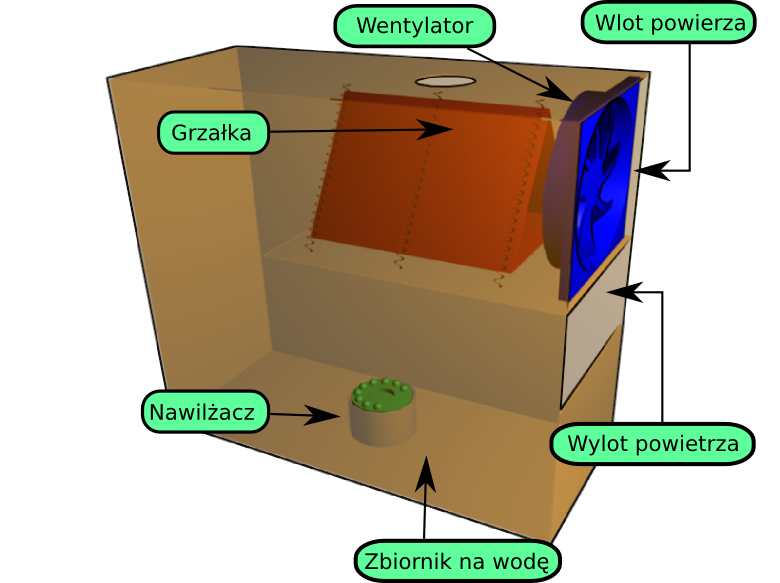
\includegraphics[width=0.9\textwidth]{figures/Wymiennik}
	\caption{Wymiennik ciepła}\label{rys:Wymiennik}
\end{figure}


% -- RURY
\subsection{Model}
Na potrzeby konkursu \emph{CSIDC} stworzono trójwymiarowy model Inkubatora, na
którym wzorowano się później przy jego konstrukcji. Końcowy wygląd urządzenia jest
bardzo zbliżony do tego przedstawionego na rysunku \ref{rys:InkubatorModel},
w~którym jednocześnie zawarto opisy najważniejszych części, co pomaga w~ich
odnalezieniu w~samym urządzeniu.

\begin{figure}[t] 
	\centering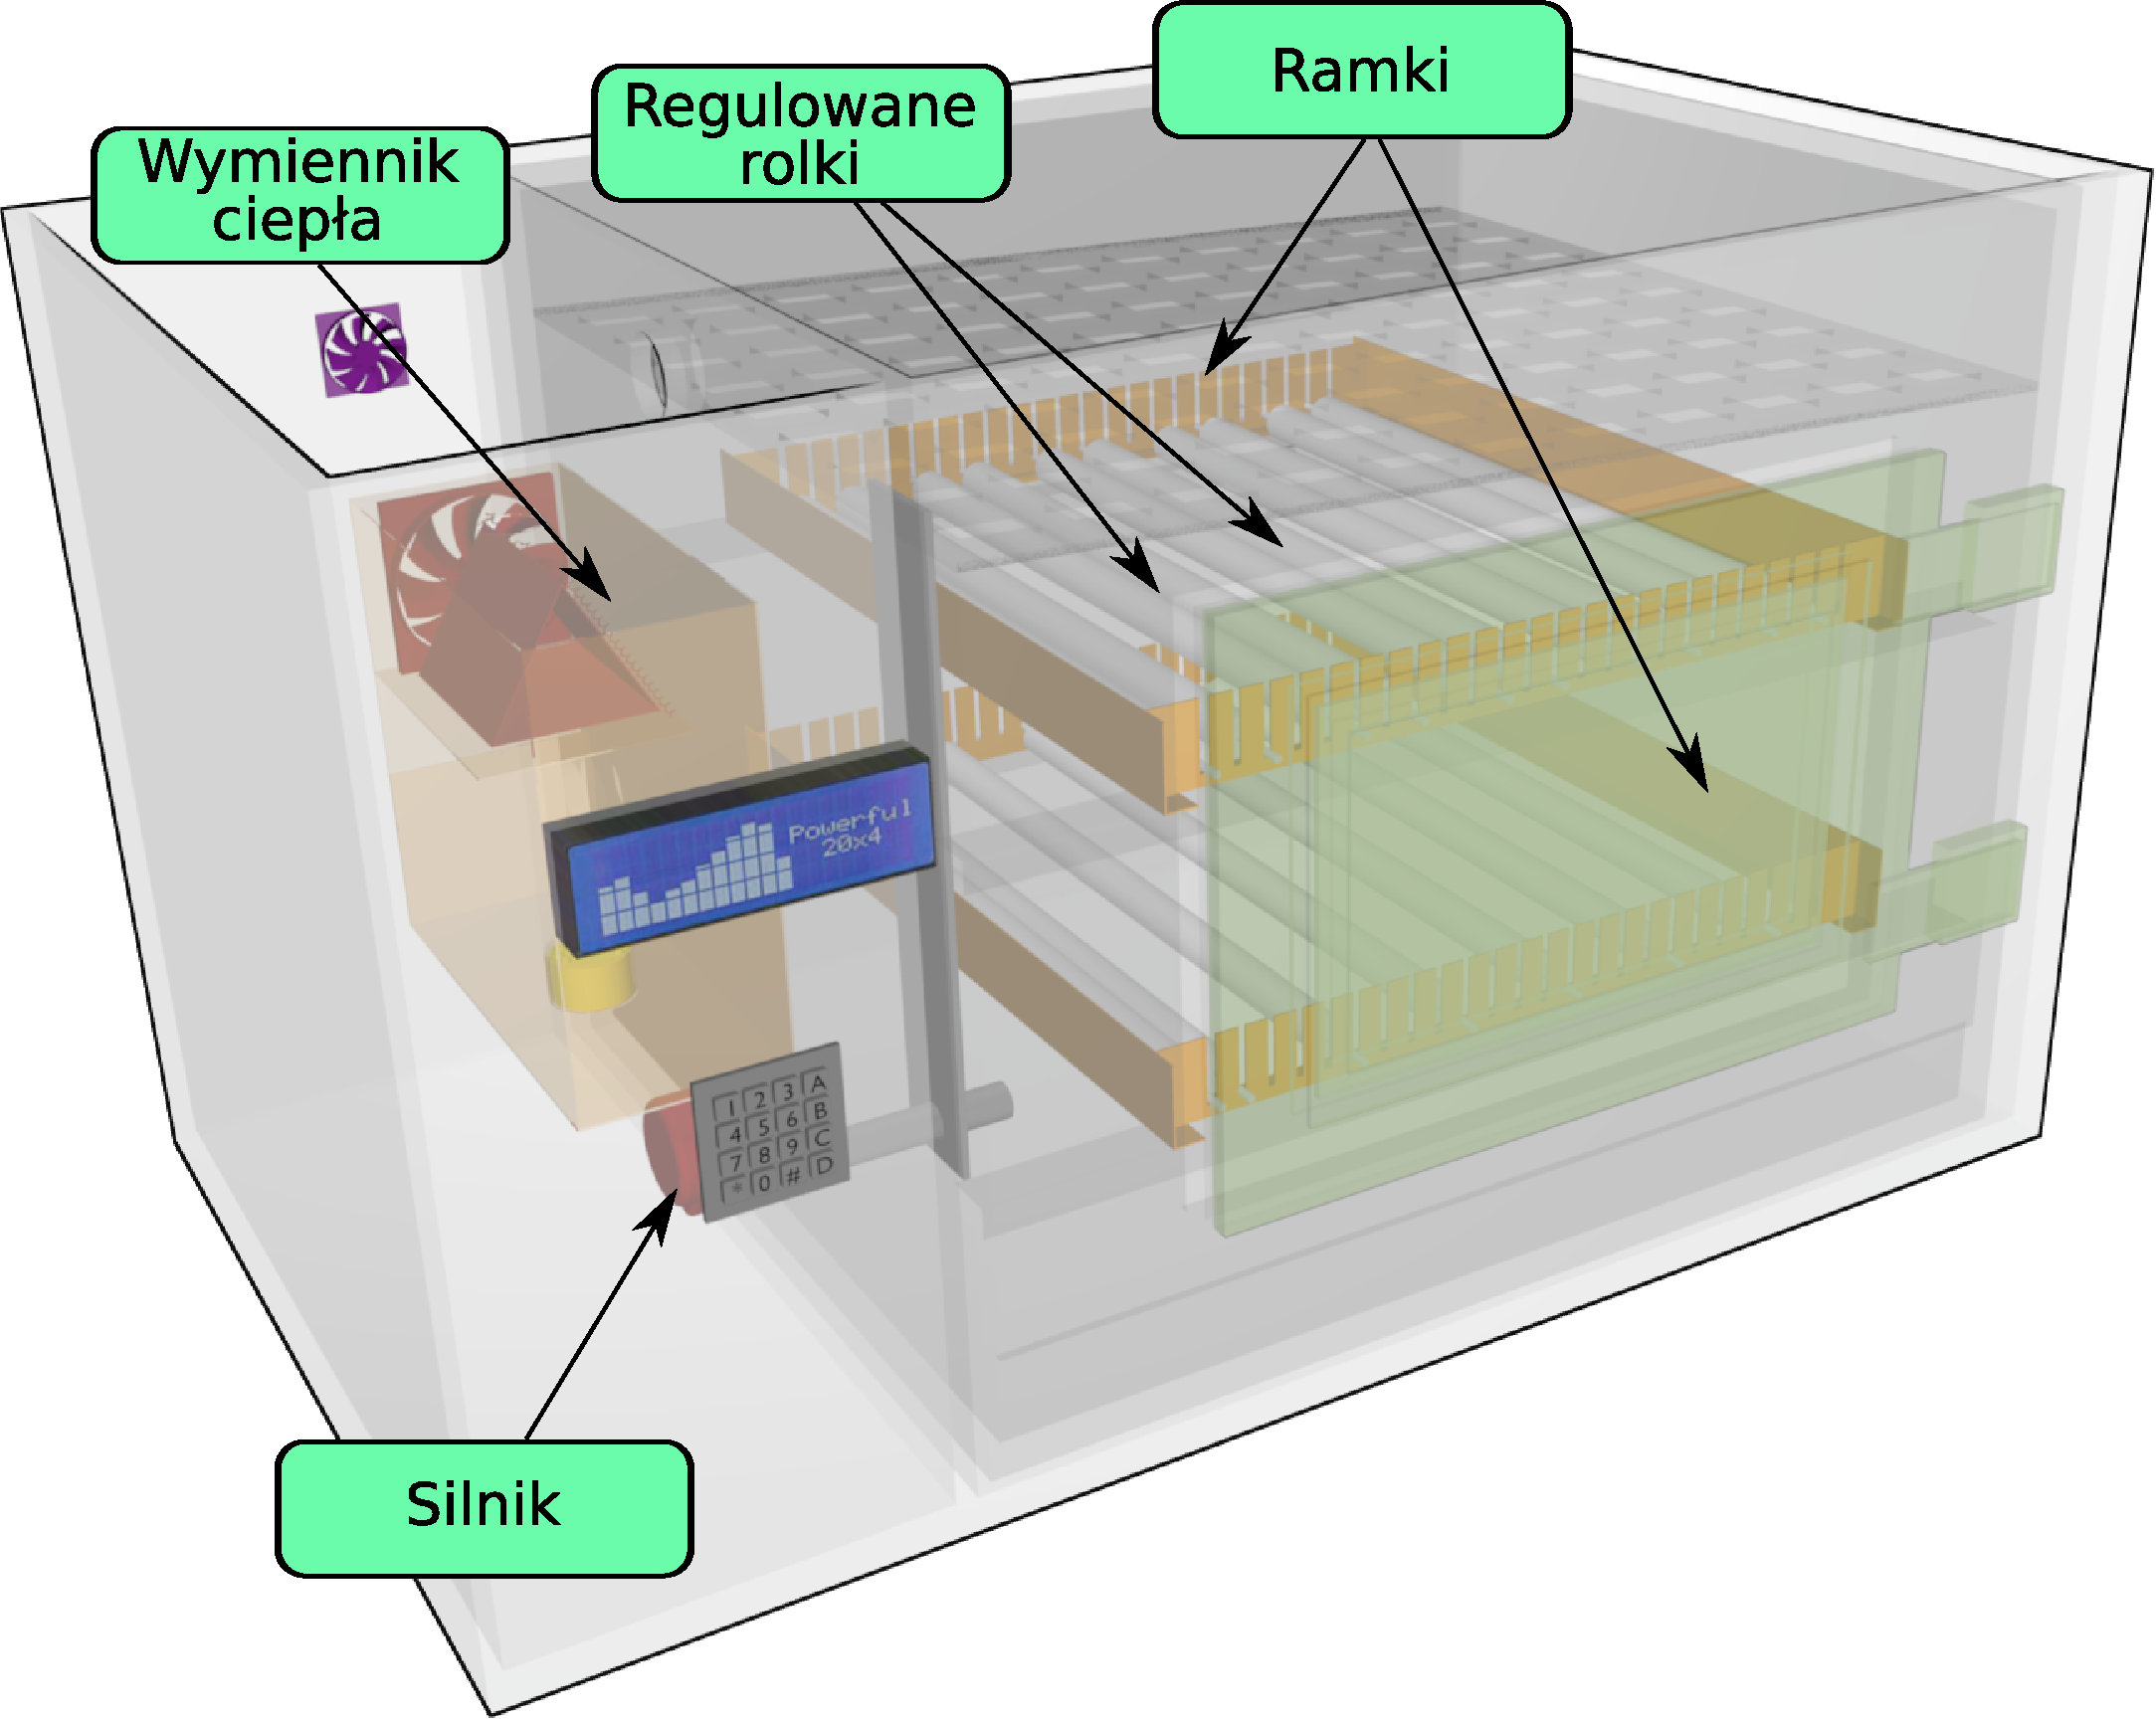
\includegraphics[width=\textwidth]{figures/Incubator}
	\caption{Model inkubatora}\label{rys:InkubatorModel}
\end{figure}

\subsection{Algorytm sterowania}
Celem algorytmu sterowania jest utrzymanie w~komorze inkubacyjnej zadanej
wartości temperatury oraz wilgotności. Do oceny jakości algorytmu sterowania
użyto średniej oraz maksymalnej wartości uchybu regulacji. Według ekspertów doskonały
inkubator powinien popełniać błąd mniejszy niż 0,1\st{} przy sterowaniu
temperaturą oraz błąd mniejszy niż 1\% przy sterowaniu wilgotnością.

Inkubator można zamodelować jako układ zamknięty ze sprzężeniem zwrotnym
\cite{Brzozka04} \cite{Bubnicki}
przedstawiony na rysunku \ref{rys:DiagramSterowania}. Bardziej szczegółowy
schemat układu ukazuje rysunek \ref{rys:SchematLogiczny}.

\begin{figure}[t] 
	\centering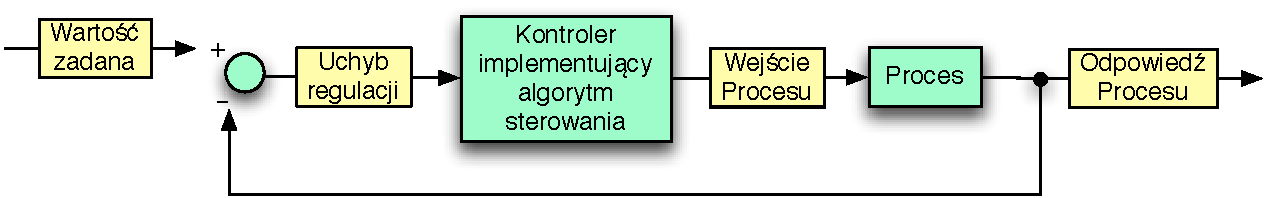
\includegraphics[width=\textwidth]{figures/DiagramSterowania}
	\caption{Układ regulacji z~logiką rozmytą}\label{rys:DiagramSterowania}
\end{figure}
	
\begin{figure}[t] 
	\centering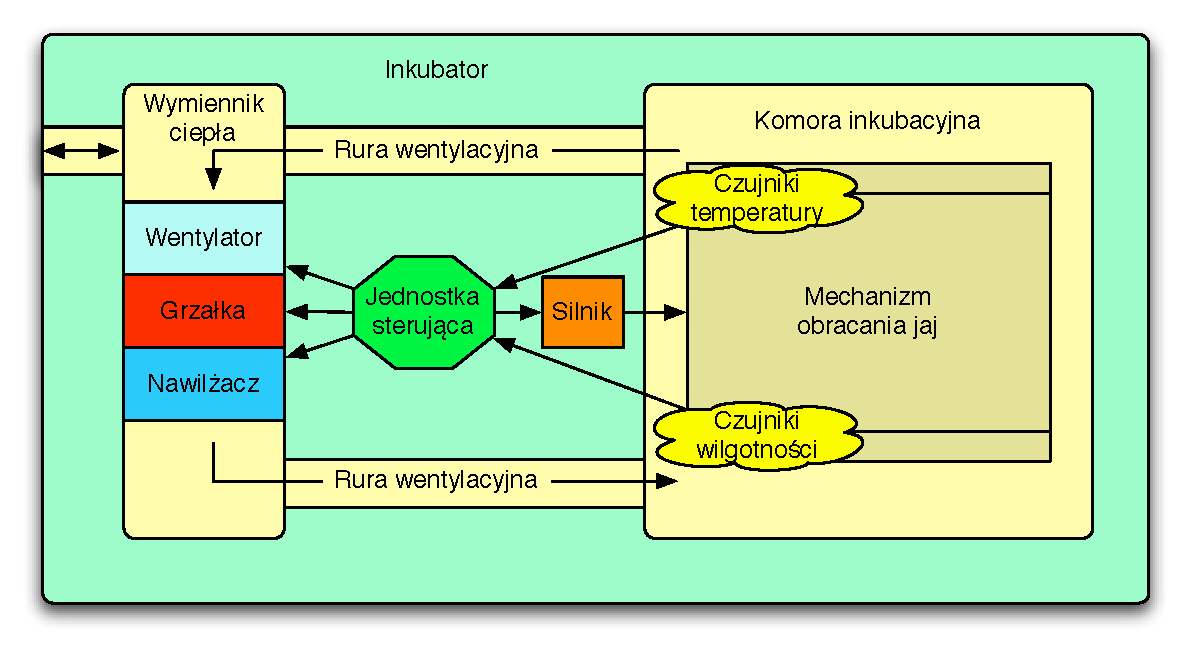
\includegraphics[width=\textwidth]{figures/SchematLogiczny}
	\caption{Schmat inkubatora}\label{rys:SchematLogiczny}
\end{figure}
	
W~fazie testowania sprzętu został zastosowany domyślny algorytm sterowania --
załącz/wyłącz. Algorytm ten dał doskonałe rezultaty przy sterowaniu wilgotnością
(dokładność 1\%) oraz przeciętne rezultaty przy sterowaniu temperaturą
(dokładność 0,8\st).

Proces jednoczesnego sterowania wilgotnością i~temperaturą jest bardzo
skomplikowany, ponieważ obie funkcje wykazują pewną korelację (np. wzrost
temperatury obniża względną wilgotność). W~przypadku inkubatora istnieją jednak
następujące podstawy by pominąć tę zależność:
\begin{itemize}
	\item przez cały czas zarówno temperatura jak i~wilgotność utrzymywane są na stałym poziomie, minimalne odchylenia jednego parametru nie mają istotnego wpływu na wartość drugiego,
	\item niezależne sterowanie temperaturą i~wilgotnością pozwala na znaczne uproszczenie modelu oraz napisanie czytelniejszego, łatwiejszego w~modyfikacji i~bardziej niezawodnego algorytmu.
\end{itemize}

Zastosowany algorytm sterowania wzorowany był na logice rozmytej \cite{FuzzyLogic} \cite{Piegat}. Wybrany został
algorytm logiki rozmytej ze względu na cechy przydatne w~zastosowaniu:
\begin{itemize}
	\item brak konieczności znajomości modelu matematycznego procesu,
	\item łatwość reprezentacji,
	\item wysoka potwierdzona doświadczalnie dokładność.
\end{itemize}

Parametrem wejściowym algorytmu sterowania jest wartość uchybu regulacji $e$
oraz jego pierwsza pochodna $\dot{e}$. Wyjście algorytmu określa sposób oddziaływania
$y =~f(e,\dot{e})$. 
%[[Dla wartości wejściowych oraz wyjściowych zdefiniowano trzy zbiory rozmyte:
%$negatywny$, $zerowy$, $pozytywny$.]]
Funkcja $f(e,\dot{e})$ jest skonstruowana jako suma ważona decyzji podejmowanej na
podstawie wartości uchybu $y_1 =~f_1(e)$ i~decyzji podejmowanej na podstawie
wartości pierwszej pochodnej uchybu $y_2 =~f_2(\dot{e})$. Funkcje $f_1$, $f_2$ mają
postać nierosnących liniowych funkcji sklejanych. Przyjmują one wartości
z~przedziału $[-1, 1]$, gdzie wartość $-1$ oznacza oddziaływanie ujemne, $0$ -- brak
oddziaływania zaś $1$ -- oddziaływanie dodatnie.
%[[maksymalną przynależność do zbioru $negatywny$, $0$ -~$zerowy$ zaś $1$ -
%$pozytywny$.]]
Intuicja podpowiada by większy wpływ na decyzję o~oddziaływaniu miała wartość
uchybu regulacji, zaś w~przypadku gdy wartość ta nie jest rozstrzygająca (czyli
bliska zeru), do głosu była dopuszczana wartość pochodnej. Zgodnie z~tym
podejściem funkcja $f(e,\dot{e})$ została zdefiniowana następująco:
\begin{equation}
f(e,\dot{e}) =~f_1(e) +~(1-|f_1(e)|) \cdot f_2(\dot{e}).
\end{equation}
Decyzja podejmowana na podstawie pochodnej uchybu $\dot{e}$ ma tym większą wagę im
mniejszą (co do wartości bezwzględnej) wartość ma funkcja $f_1$. Początkowo
przebieg funkcji sklejanych $f_1$ i~$f_2$ został ustalony arbitralnie. Algorytm
sterowania temperaturą dawał wówczas dokładność sterowania rzędu 0,5\st. Wynik
ten był lepszy od wyniku algorytmu załącz/wyłącz, co potwierdziło użyteczność
przyjętego algorytmu. Seria dalszych eksperymentów pozwoliła na taki dobór
funkcji $f_1$ i~$f_2$, by błąd sterowania temperaturą mieścił się w~granicach
0,1\st. Wynik ten jest najlepszym z~wyników możliwych do osiągnięcia, zwłaszcza że wartość
0,1 stanowi maksimum uchybu regulacji, zaś średni uchyb jest niemalże równy
zeru. Ostateczną postać liniowych funkcji sklejanych $y_1 =~f_1(e)$
i~$y_2~=f2(\dot{e})$, uzyskanych drogą empiryczną przedstawiają
rysunki~\ref{rys:t_zygzaczek} i~\ref{rys:dt_zygzaczek}.

%[[wektor ma zrobić wykresy liniowych funkcji sklejanych]]

\begin{figure}[p] 
	\centering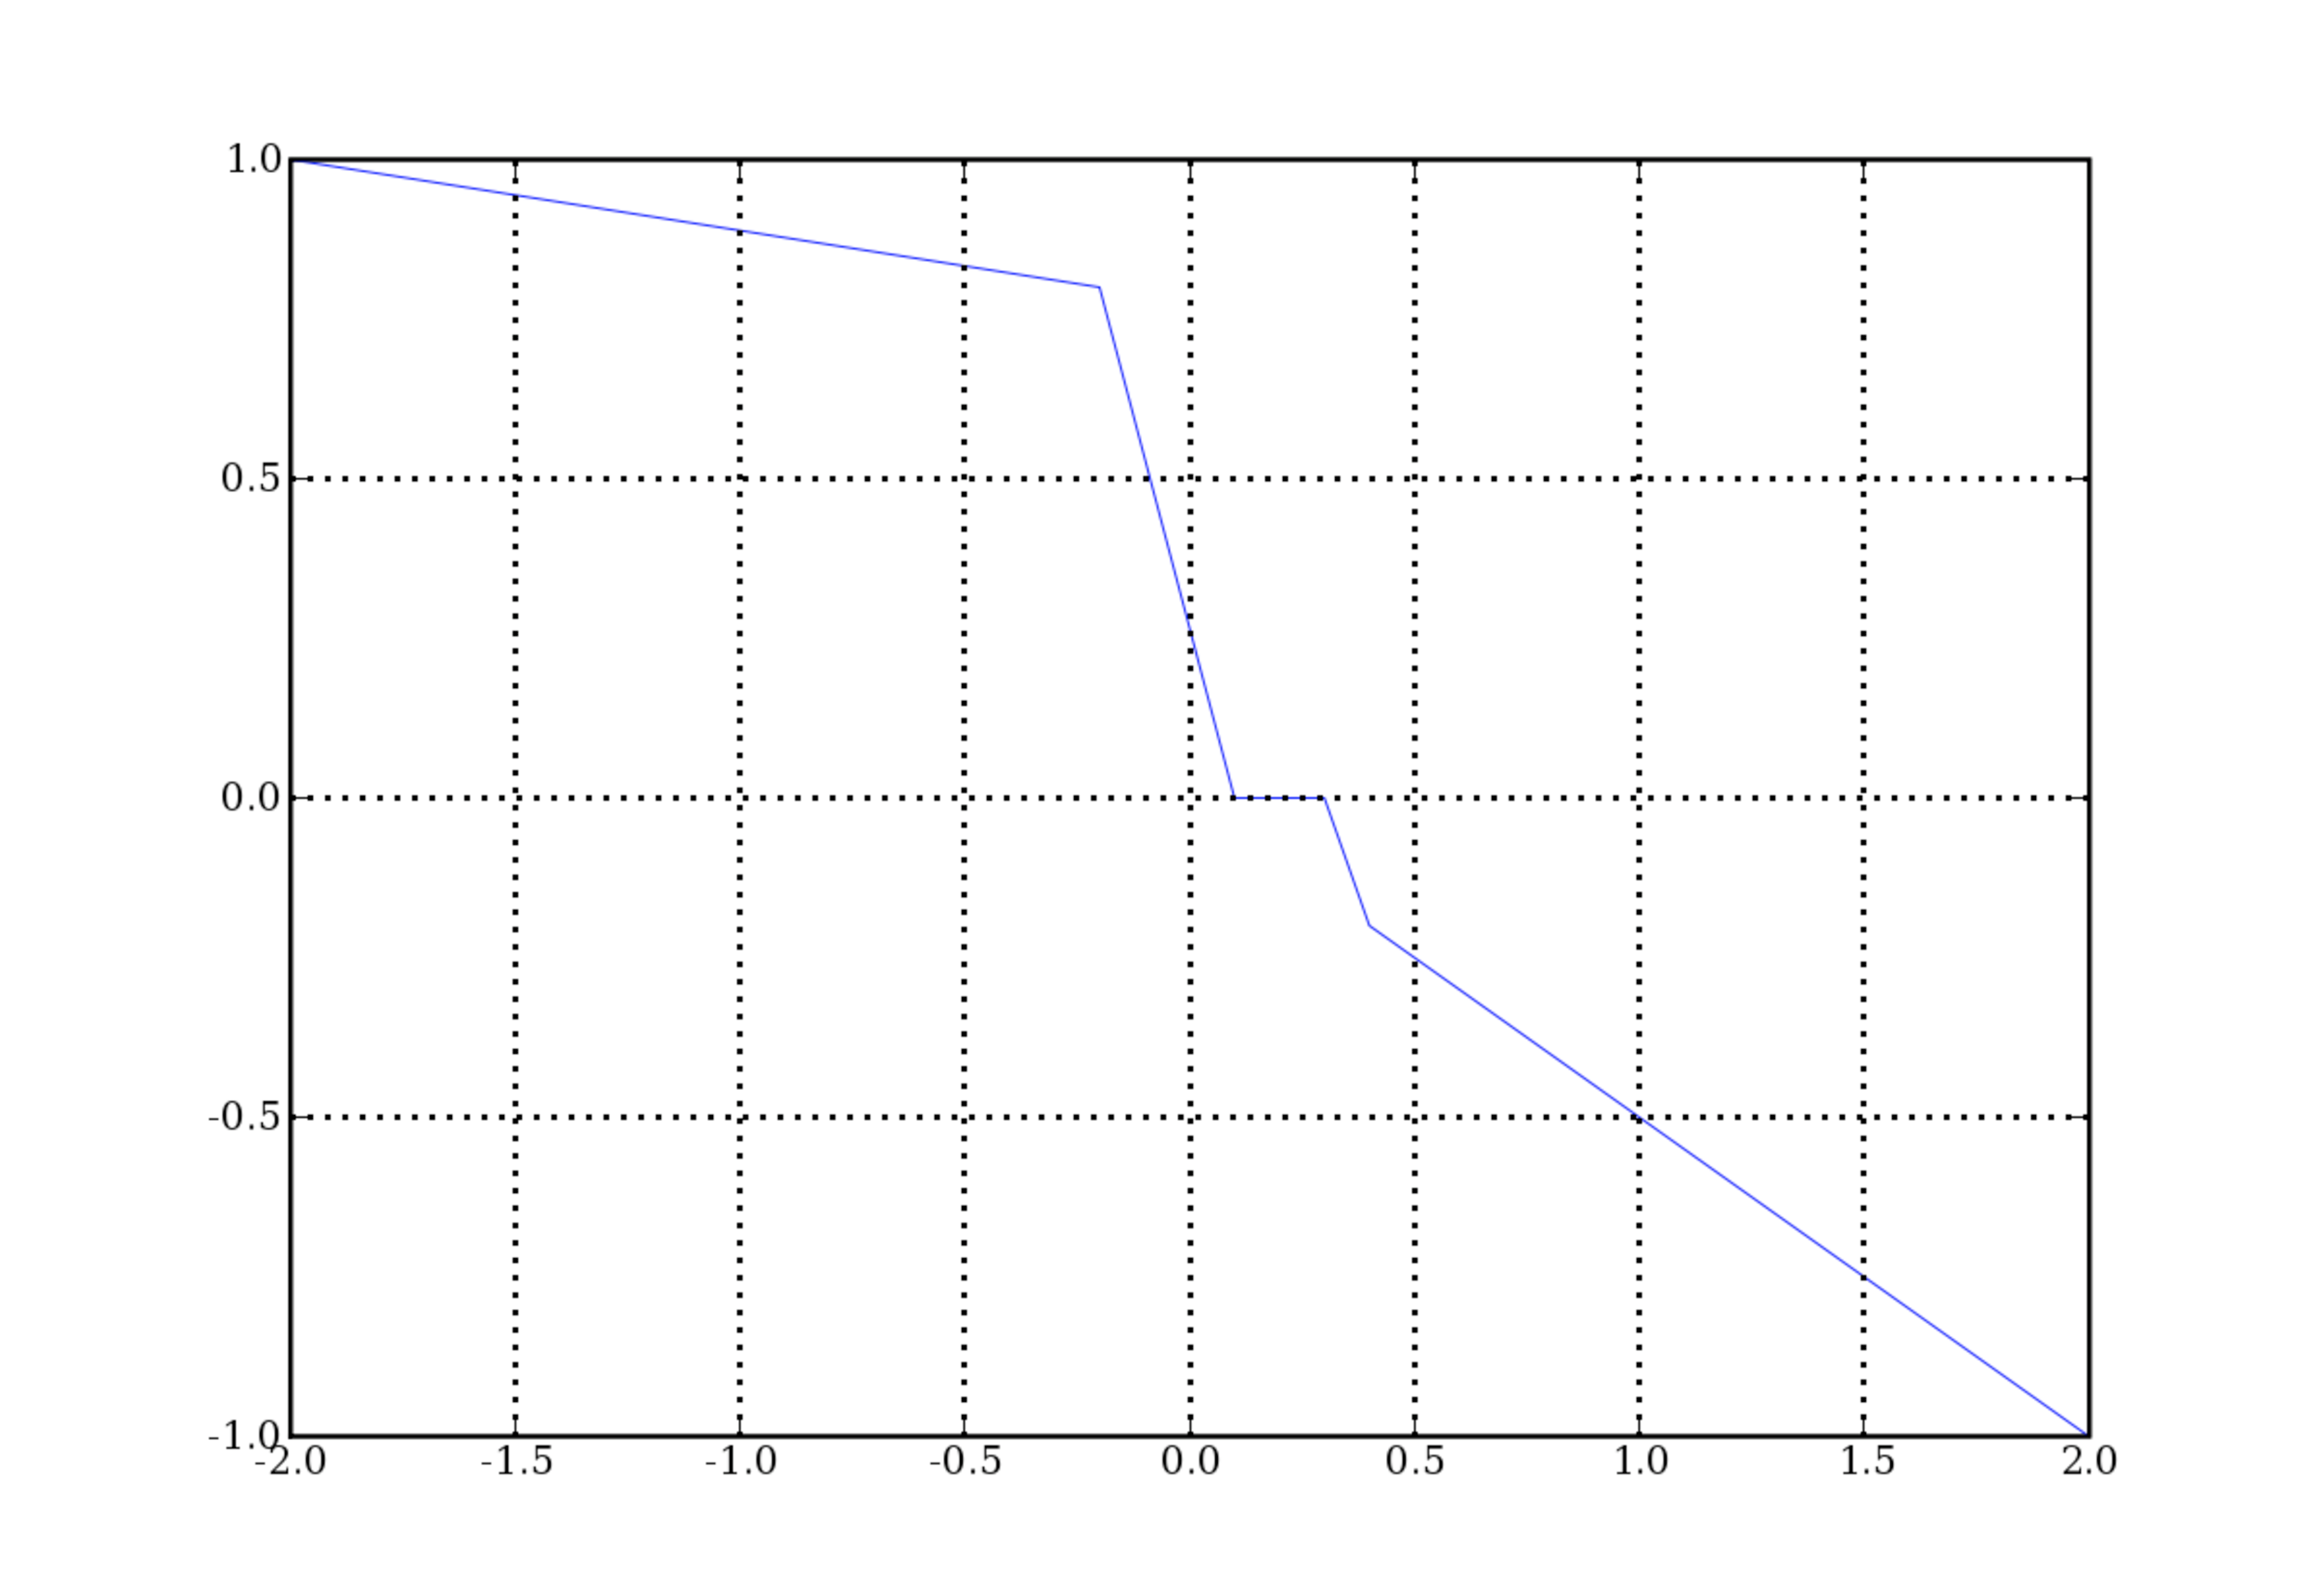
\includegraphics[width=\textwidth]{figures/t_zygzaczek}
	\caption{Odpowiedź względem temperatury ($f_1(e)$)}\label{rys:t_zygzaczek}
\end{figure}

\begin{figure}[p] 
	\centering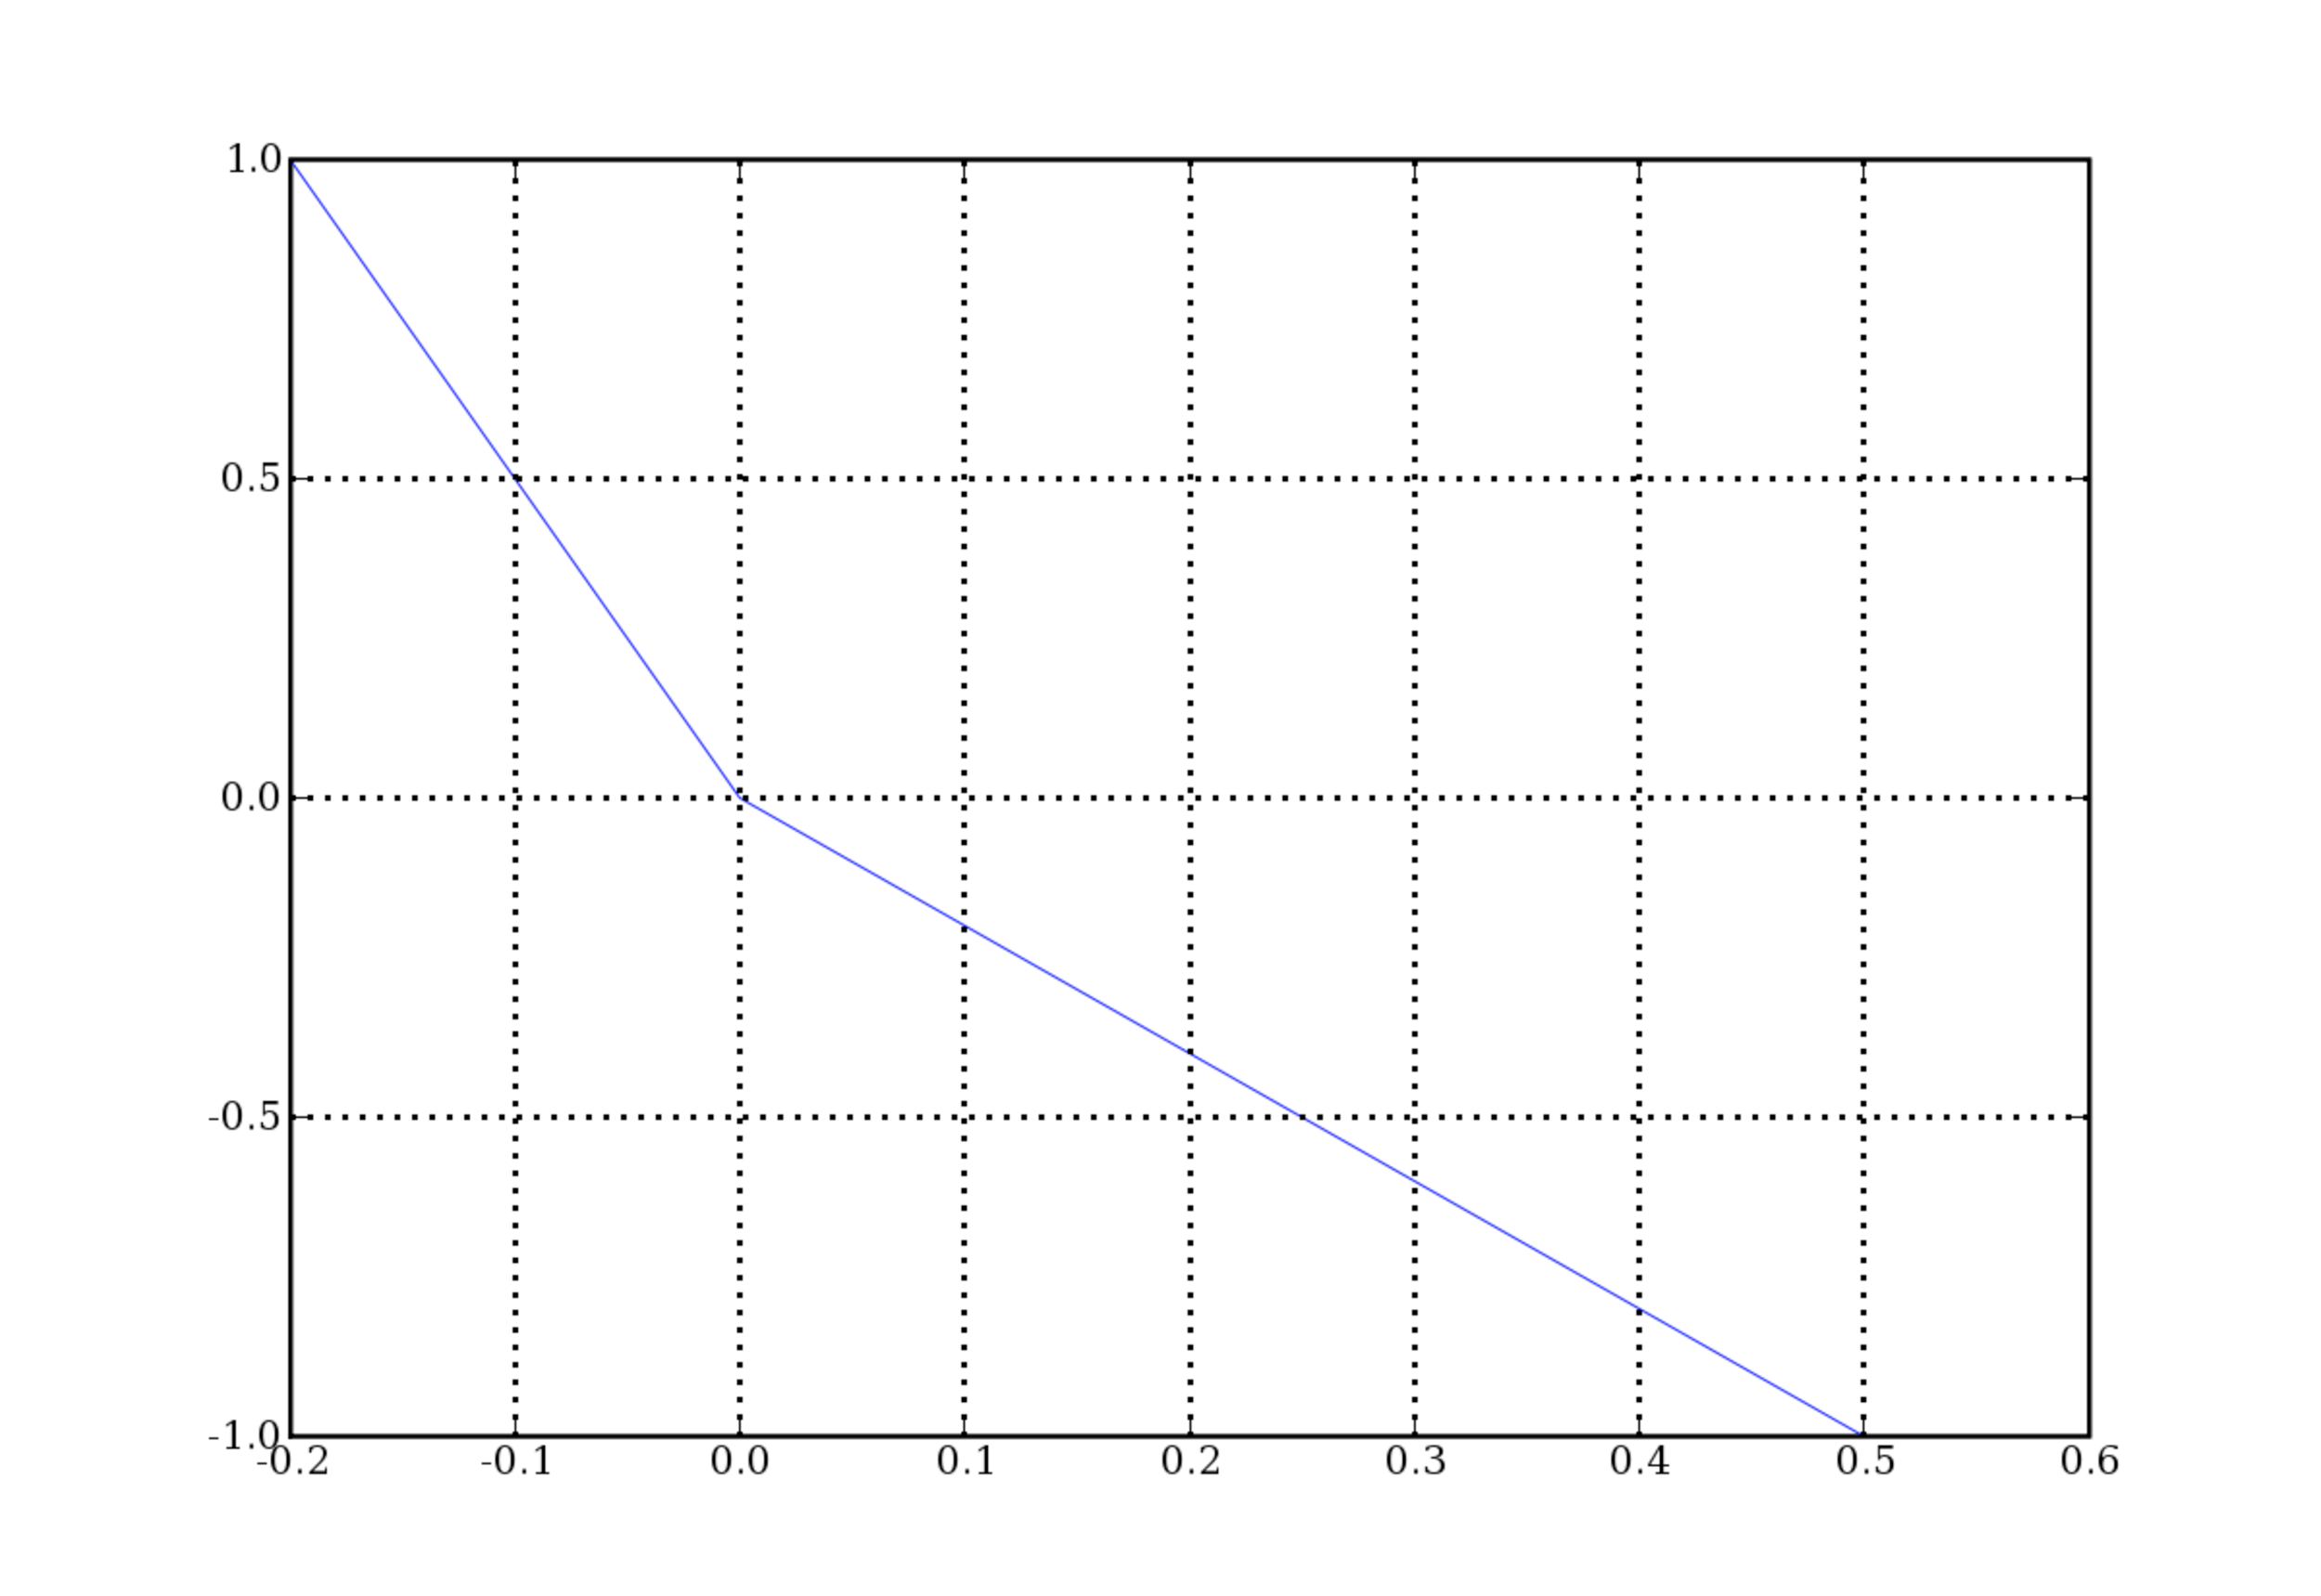
\includegraphics[width=\textwidth]{figures/dt_zygzaczek}
	\caption{Odpowiedź względem zmiany temperatury ($f_2(\dot{e})$)}\label{rys:dt_zygzaczek}
\end{figure}

Odpowiedź algorytmu w~całej dziedzinie argumentów przedstawiona jest
na rysunku \ref{rys:sterowanie3d}.

\begin{figure}[t] 
	\centering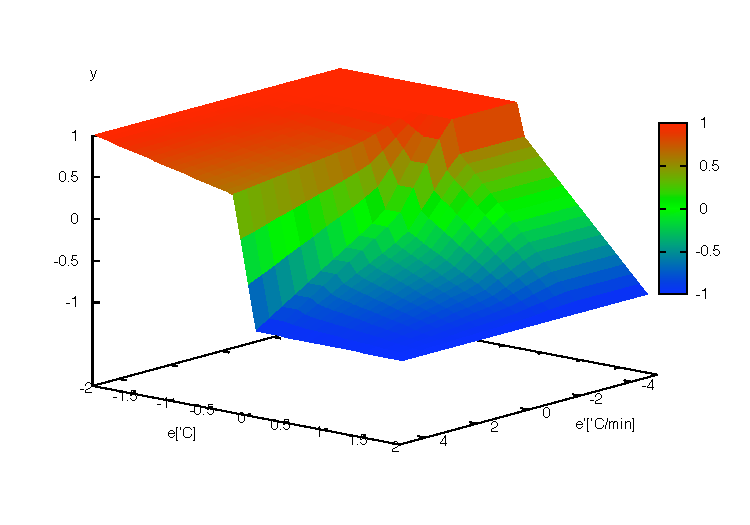
\includegraphics[width=16cm]{figures/sterowanie3d}
	\caption{Odpowiedź w~całej dziedzinie, rzut 3d ($f(e, \dot{e})$)}\label{rys:sterowanie3d}
\end{figure}

Opisany algorytm został zastosowany do sterowania temperaturą, natomiast do
sterowania wilgotnością wykorzystano sprawdzony wcześniej algorytm załącz/wyłącz.
W implementacji oba algorytmy rejestrują wartości uchybów co $w$ sekund oraz
podejmują decyzję co $n \cdot w$ sekund. Wartość uchybu ($e$) wykorzystywana na wejściu
algorytmu sterowania obliczana jest jako średnia z~ostatnich trzech zmierzonych
uchybów, wartość pochodnej uchybu ($\dot{e}$) jest obliczana jako różnica między
średnią z~trzech ostatnich uchybów i~średnią z~trzech poprzednich uchybów.

\subsection{Elektronika}
Prawidłowy przebieg inkubacji zapewnia komputer pokładowy. Spełnia on poniższe wymagania:
\paragraph{Niezawodność.} 
Po przeprowadzeniu rozpoznania wybrano komputer PCM-9575 produkowany przez firmę
Advantech. Jest to tzw. ,,Single Board Computer'' formatu EBX 5,25 cala
z~procesorem VIA Embedded Eden 400MHz, którego wydajność w~zupełności wystarcza.
Komputer ten może działać bez wentylatora w~temperaturach do 60\st, co pozwala
działać mu bezawaryjnie w~warunkach wewnątrz inkubatora. Wbudowany interfejs
VGA/LCD pozwala podłączyć monitor i~bezpośrednio obserwować działanie algorytmów
i~stan procesów, a~także wprowadzać poprawki w~sposób interaktywny.

\paragraph{Wysoka wydajność.}
Uruchomienie wielu osobnych procesów wymaga odpowiedniej mocy obliczeniowej oraz
odpowiedniej ilości pamięci RAM. Procesor ma zapas mocy która może okazać się
potrzebna w~przypadku wprowadzenia dodatkowej funkcjonalności. Rozmiar pamięci
operacyjnej -- 128 MB jest szczególnie istotny, ponieważ w~trakcie działania
aplikacji większość operacji odczytu i~zapisu przeprowadzanych jest na
wirtualnym systemie plików właśnie w~pamięci operacyjnej, celem zminimalizowania
liczby operacji odczytu i~zapisu na karcie pamięci CompactFlash.

\paragraph{Minimalny koszt wdrożenia.}
W celu obniżenia kosztu wdrożenia Thinkubatora do ogrodów zoologicznych
zadecydowano o~użyciu połączeń ethernetowych. Polskie ogrody są już podłączone do
internetowego systemu inwentaryzowania zwierząt ISIS (\emph{http://www.isis.org}),
zatem infrastruktura sieciowa jest gotowa do użycia.

\paragraph{Rozszerzalność.}
Thinkubator znajduje się obecnie na etapie prototypu. Możliwość podłączenia
dysków EIDE lub urządzeń USB umożliwia rozszerzanie systemu o~standardowe
komponenty. Korzystając z~interfejsu PC/104-Plus komputer pokładowy można
dowolnie rozszerzać o~specjalistyczne urządzenia, które mogą mieć zastosowanie
w~ogrodach zoologicznych ze specjalnymi wymaganiami.

\paragraph{Łatwość rozwijania.}
Komputer posiada wbudowany czytnik kart typu CompactFlash. Na przygotowanej karcie CompactFlash
o~pojemności 256MB znajduje się system i~pliki konfiguracyjne, a~także partycja
służąca za nieulotną pamięć do zapisu. Gdy połączenie Ethernet jest niedostępne,
historia inkubacji jest zapisywana na karcie, którą można następnie odczytać na
zwykłym komputerze PC i~przesłać do Centrum Nadzoru.

Sterowanie środowiskiem opera się na sprzężeniu zwrotnym. Zastosowano kilka
rodzajów czujników. Do pomiaru wilgotności zdecydowano się na użycie
zintegrowanego czujnika wilgotności i~temperatury Dallas Hygrochron ze względu
na jego wysoką precyzję (0,6\%RH) oraz możliwość łatwej komunikacji cyfrowej. Do
produkcji seryjnej przewiduje się dużo tańsze czujniki pojemnościowe, jednak dla
celów przejrzystości w~prototypie stosowano rozwiązania pewne i~sprawdzone.
Pomiary przekazywane są poprzez magistralę szeregową 1-wire.

Do tej samej magistrali podłączono trzy czujniki temperatury serii DS1820.
Zastosowanie tradycyjnego termostatu było wykluczone ze względu na konieczność
centralnego sterowania środowiskiem z~komputera. Zmierzona wartość temperatury
wyświetlana jest na ekranie ciekłokrystalicznym. Eliminuje to konieczność
umieszczenia termometru rtęciowego w~komorze inkubacyjnej i~wiążącego się z~tym
zagrożenia zatruciem tlenkami rtęci w~przypadku uszkodzenia.

Czujniki podłączone są do opracowanej przez Dallas Semiconductors szyny 1-wire.
Używa ona jedynie dwóch przewodów, jednego do zasilania i~przesyłania sygnałów,
drugiego do masy, dzięki czemu jest bardzo łatwa we wprowadzeniu i~rozbudowie.
Można do niej podłączyć dużą liczbę różnych urządzeń, m.in. czujników,
adresowalnych przełączników, potencjometrów cyfrowych. W~Inkubatorze
wykorzystano samodzielnie zbudowany adapter podłączany do portu RS-232. 
Schemat ideowy adaptera widoczny jest na rysunku \ref{rys:Adapter}.

\begin{figure}[t] 
\centering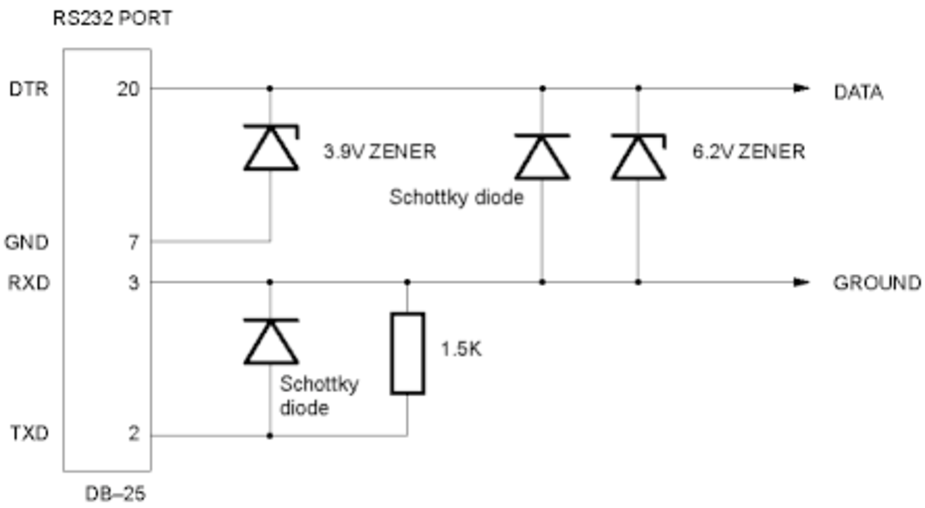
\includegraphics[width=\textwidth]{figures/adapter}
\caption{Adapter 1-wire}\label{rys:Adapter}
\end{figure}

Interfejs użytkownika inkubatora składa się z~niebiesko-białego wyświetlacza
ciekłokrystalicznego zawierającego po 20 znaków w~2 rzędach
oraz klawiatury z~16 guzikami podłączonej do portu \emph{PS/2}. Ekran podłączony
jest do portu równoległego komputera w~trybie 4-bitowym.

Sygnały z~komputera są wyprowadzone poprzez port równoległy. Oświetlenie komory
lęgowej wykonano przy użyciu diod LED, zapewniając wysoką trwałość systemu
oświetlenia i~umożliwiając nieskrępowane załączanie i~wyłączanie oświetlenia bez
wprowadzania wahań temperatury. Diody są załączane poprzez tranzystor, natomiast trzy
urządzenia wykonawcze są włączane przez płytkę z~przekaźnikami.

Grzałka na 230V jest podłączona do przekaźnika, który załącza napięcie w~odpowiednim momencie.

Nawilżacz jest również załączany poprzez przekaźnik. Potrzebny mu zasilacz 24V
prądu zmiennego jest podłączony do wejścia 220V wewnątrz części technicznej inkubatora.

Silnik do przesuwania rolek jest podłączony do źródła napięcia 220V
i~uruchamiany za pomocą przekaźnika.

\subsection{Aplikacja sterująca}
Architektura aplikacji sterującej inkubatorem oparta jest na grupie niezależnych
procesów komunikujących się ze sobą za pomocą segmentu pamięci współdzielonej.
Procesy zostały zaprojektowane w~taki sposób, aby nie nie wymagały silnego
zarządzania współbieżnością, ponieważ każdy z~nich wykonuje własne unikatowe
operacje. Interakcje pomiędzy procesami zostały przedstawione na rysunku
\ref{rys:SHM}.

\begin{figure}[t] 
\centering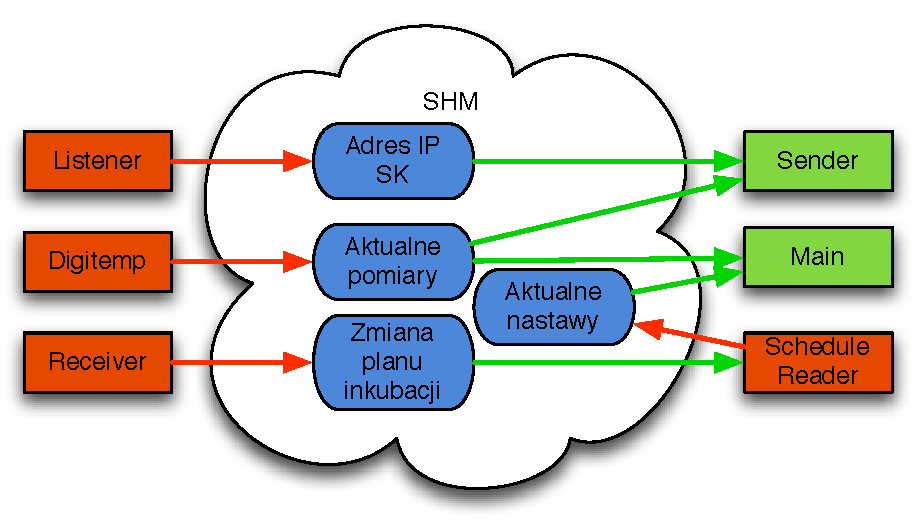
\includegraphics[width=\textwidth]{figures/SHM}
\caption{Schemat procesów}\label{rys:SHM}
\end{figure}

Proces \textbf{Main} jest najważniejszą częścią aplikacji. Korzysta
z~wszystkich informacji zbieranych przez inne procesy i~na ich podstawie podejmuje
decyzje o~uruchamianiu odpowiednich urządzeń wykonawczych w~celu najlepszego
odwzorowania planu inkubacji wewnątrz inkubatora. Jest podzielony na dwie główne
części: moduł abstrakcji sprzętowej, czyli zaimplementowane funkcje włączające
i~wyłączające urządzenia oraz algorytm sterowania, który do poprawnego działania
potrzebuje dwóch informacji. Pierwszą są aktualne parametry komory inkubacyjnej
-- temperatura i~wilgotność, za zbieranie których odpowiedzialny jest proces
\textbf{Digitemp} -- adaptacja otwartego programu o~tej samej nazwie służącego
do odczytywania informacji z~czujników 1-wire; drugą -- parametry inkubacji
nastawione przez operatora urządzenia. Dostarcza je proces \textbf{Schedule
Reader}, którego zadaniem jest także wczytywanie nowego planu inkubacji, jeśli ten
zostanie zmieniony w~trakcie jej trwania. \textbf{Sender} jest odpowiedzialny za
cykliczne wysyłanie informacji na temat stanu inkubacji do \emph{Stacji
Kontrolnej} oraz \emph{Centrum Nadzoru}, natomiast \textbf{Receiver} nasłuchuje
ruch sieciowy i~odpowiada na wszystkie wiadomości wysłane do inkubatora za
wyjątkiem sygnału rozgłoszeniowego wyszukującego inkubatory -- za tę czynność
odpowiedzialny jest \textbf{Listener}.

Dodatkowo działają dwa procesy związane z~interfejsem zamontowanym na
inkubatorze -- wyświetlaczem LCD oraz klawiaturą. 

Proces keyboardd oczekuje na sygnały z~klawiatury. Wykorzystywana jest metoda
"poll". Poprzez załączanie napięcia na kolejnych liniach szyny poziomej
i~odczytywanie stanu poszczególnych linii szyny pionowej otrzymujemy bieżący stan
klawiatury. Po zmianie stanu jednej z~odczytywanych linii na wysoki i~powrotu do
stanu niskiego wprowadzony znak jest rozpoznawany i~umieszczany w~kolejce FIFO
/dev/kbd.

Proces displayd prezentuje na wyświetlaczu LCD przede wszystkim bieżący stan
środowiska wewnątrz inkubatora. W~przypadku problemów wyświetla informacje
o~zaistniałym zagrożeniu i~podaje źródło, z~którego można zasięgnąć informacji
które będą służyły rozwiązaniu problemu. Ekran ciekłokrystaliczny stanowi też ważny
komponent systemu sterowania inkubatorem: wyświetla złożony system menu,
pozwalający na konfigurację, zaawansowany monitoring oraz wykonywanie
czynności serwisowych.

Przez większość czasu proces oczekuje na operację odczytu z~kolejki FIFO.
Jednocześnie program wykorzystuje mechanizm sygnałów, aby obsłużyć zdarzenia z~innych
źródeł. Przykładowo, czas na zaktualizowanie wyświetlanej temperatury jest
sygnalizowany co sekundę poprzez dostarczenie SIGALRM zamówionego przy pomocy
funkcji systemowej alarm. Po nadejściu sygnału (czas zaktualizowania
wyświetlanej temperatury, otwarcie drzwiczek, itd.) program przechodzi do jego
obsługi i~wraca oczekiwać na nowy znak. Przez cały ten czas na wyświetlaczu
widać bieżącą temperaturę i~wilgotność lub bieżący wycinek systemu menu -- listę
opcji, zachętę do wprowadzenia nowej temperatury czy potwierdzenie operacji
wyłączenia inkubatora.

Diagram przejść stanów programu obsługi wyświetlacza znajduje się na
rysunku~\ref{rys:Menu}. Przedstawia on zaimplementowany schemat menu, jego
strukturę oraz działanie. Stanowi równocześnie ważną część instrukcji obsługi
inkubatora.


\begin{figure}[b] 
\centering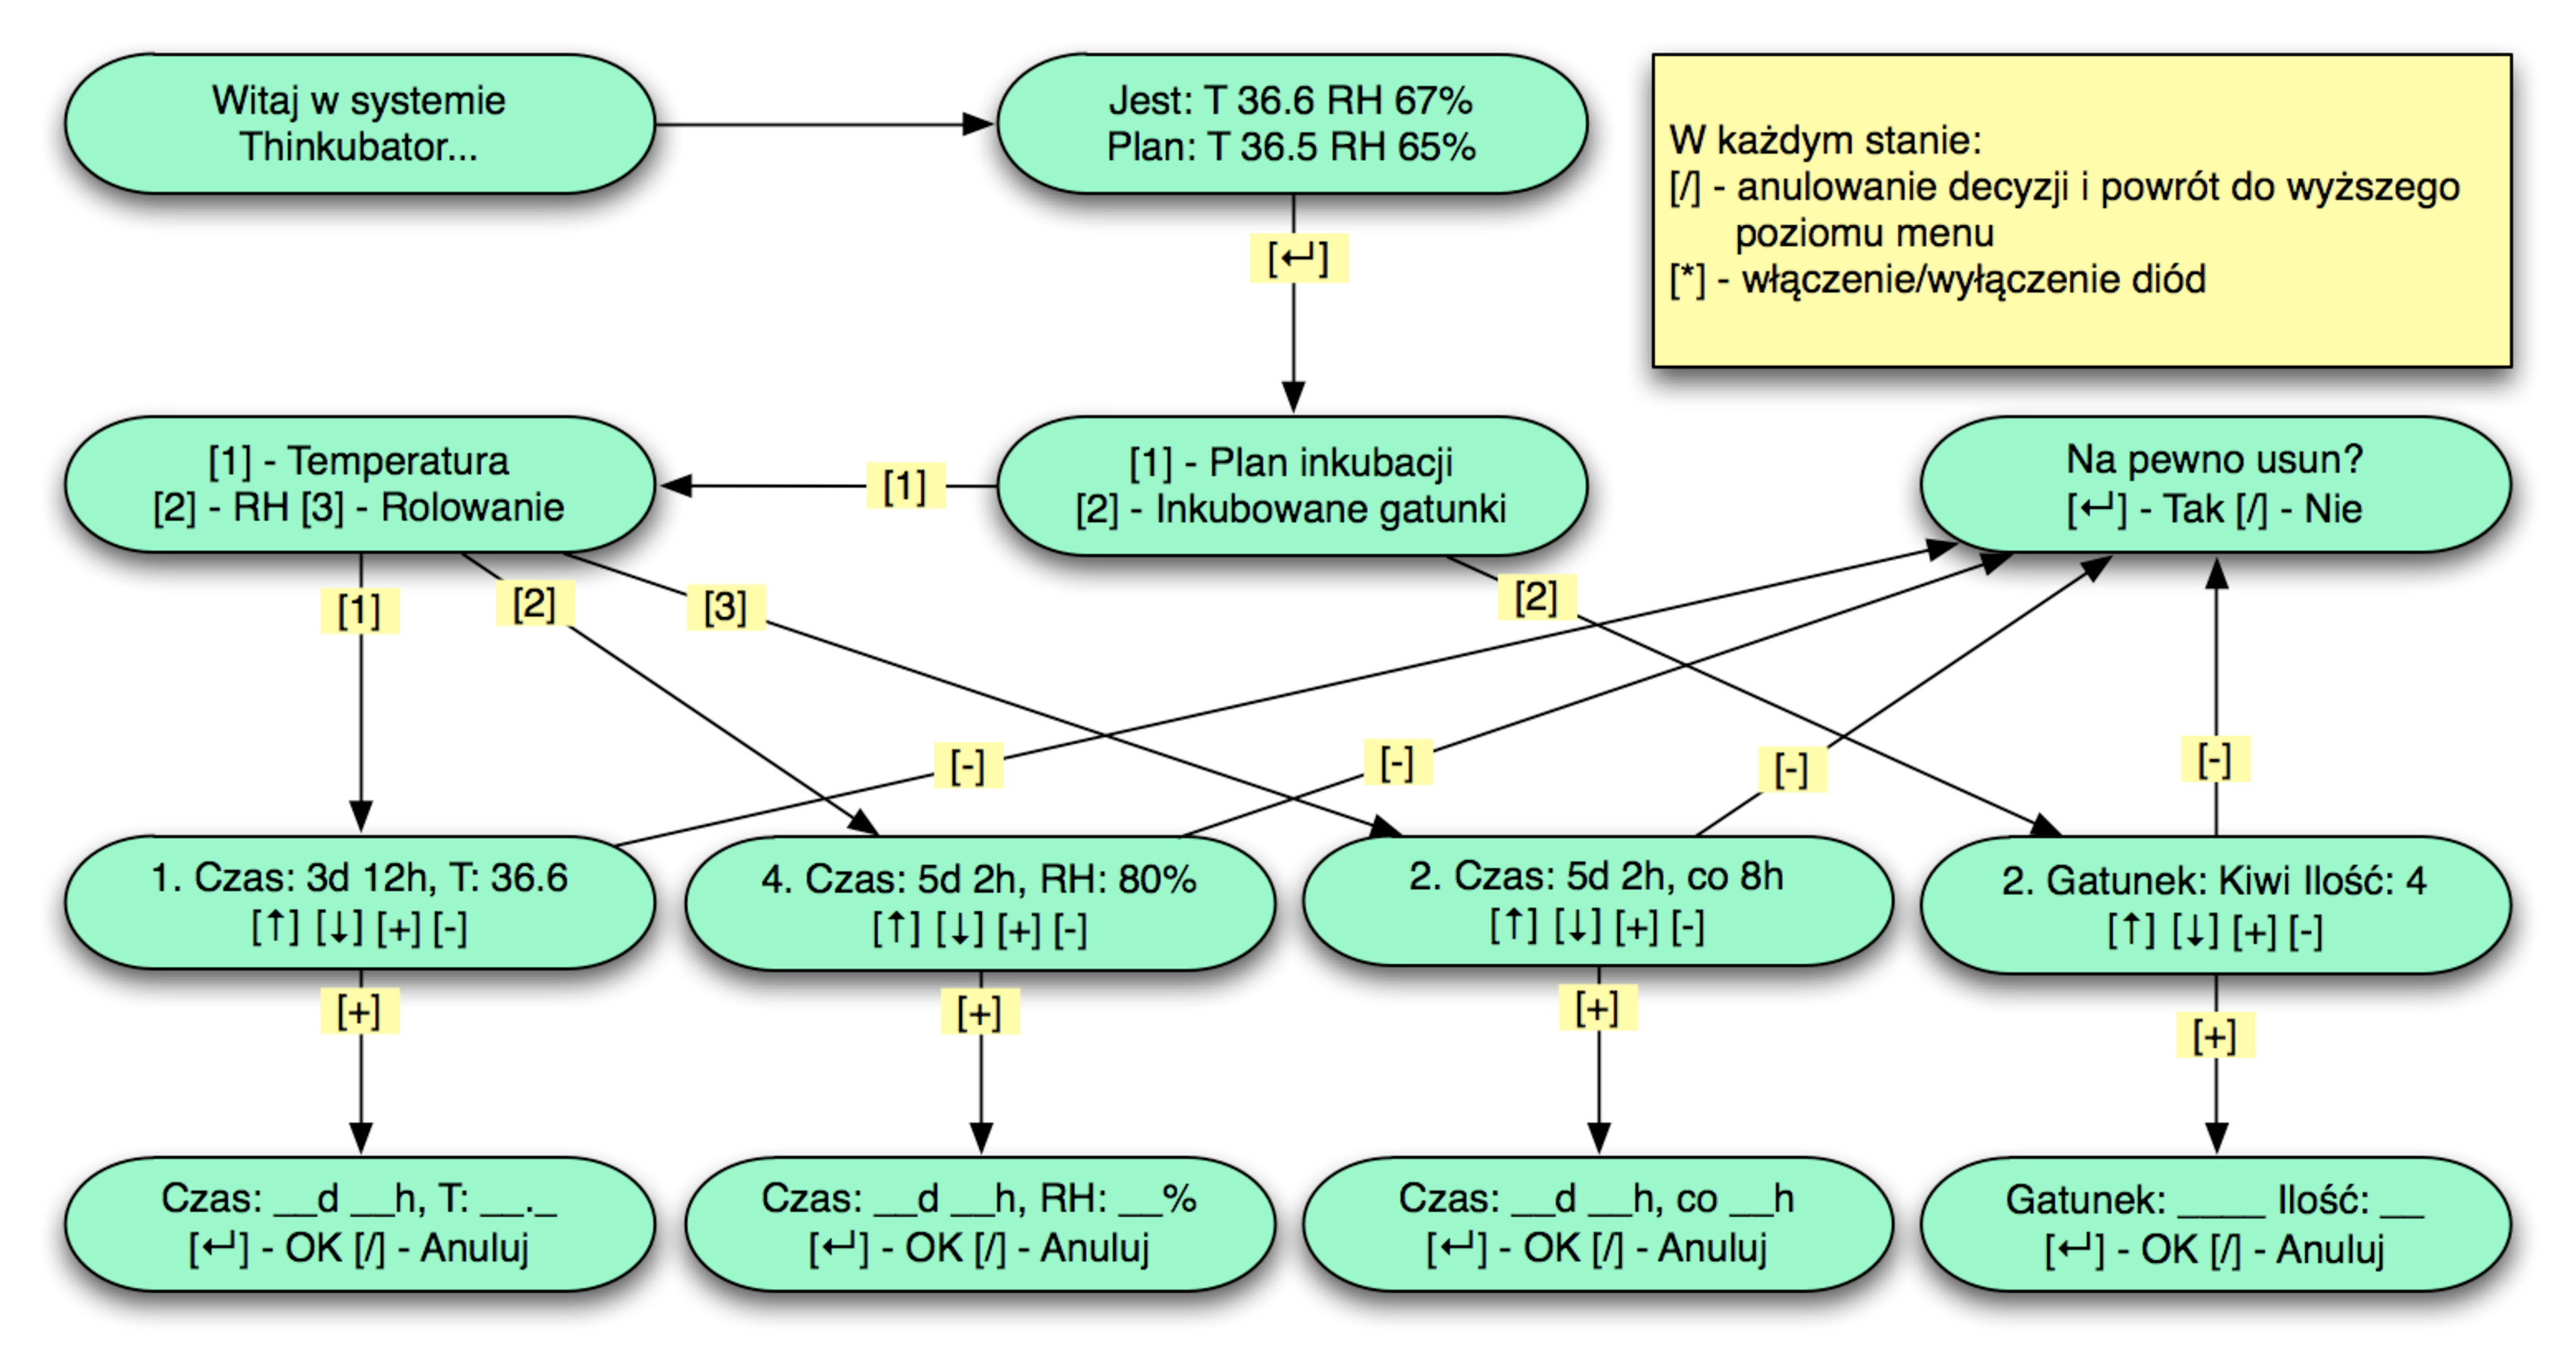
\includegraphics[width=\textwidth]{figures/Menu}
\caption{Diagram menu}\label{rys:Menu}
\end{figure}

\subsection{System operacyjny}
Aplikacja została zaimplementowana na system operacyjny Linux. Wybrano ten
system operacyjny gdyż potrzebowano pełnowymiarowego systemu operacyjnego, który
zapewniłby:
\begin{itemize}
 \item stos TCP/IP,
 \item kontrolę nad współbieżnością,
 \item biblioteki zapewniające dogodny dostęp do portów i~protokołów komunikacyjnych.
\end{itemize}
Wybór padł właśnie na system Linux, ponieważ dodatkowo:
\begin{itemize}
 \item ma silne środowisko do implementacji,
 \item zapewnia łatwość rekonfiguracji systemu -- dostosowanie systemu do posiadanej platformy sprzętowej,
 \item jest dobrze znany członkom zespołu.
\end{itemize}

\section{Komunikacja}
Ogólny przebieg komunikacji pomiędzy elementami systemu przedstawia
rysunek~\ref{rys:Komunikacja}. Linie czerwone oznaczają połączenia nawiązywane
za pomocą gniazd BSD, zielone -- XML-RPC, czarne -- HTTP.
\begin{figure}[b] 
\centering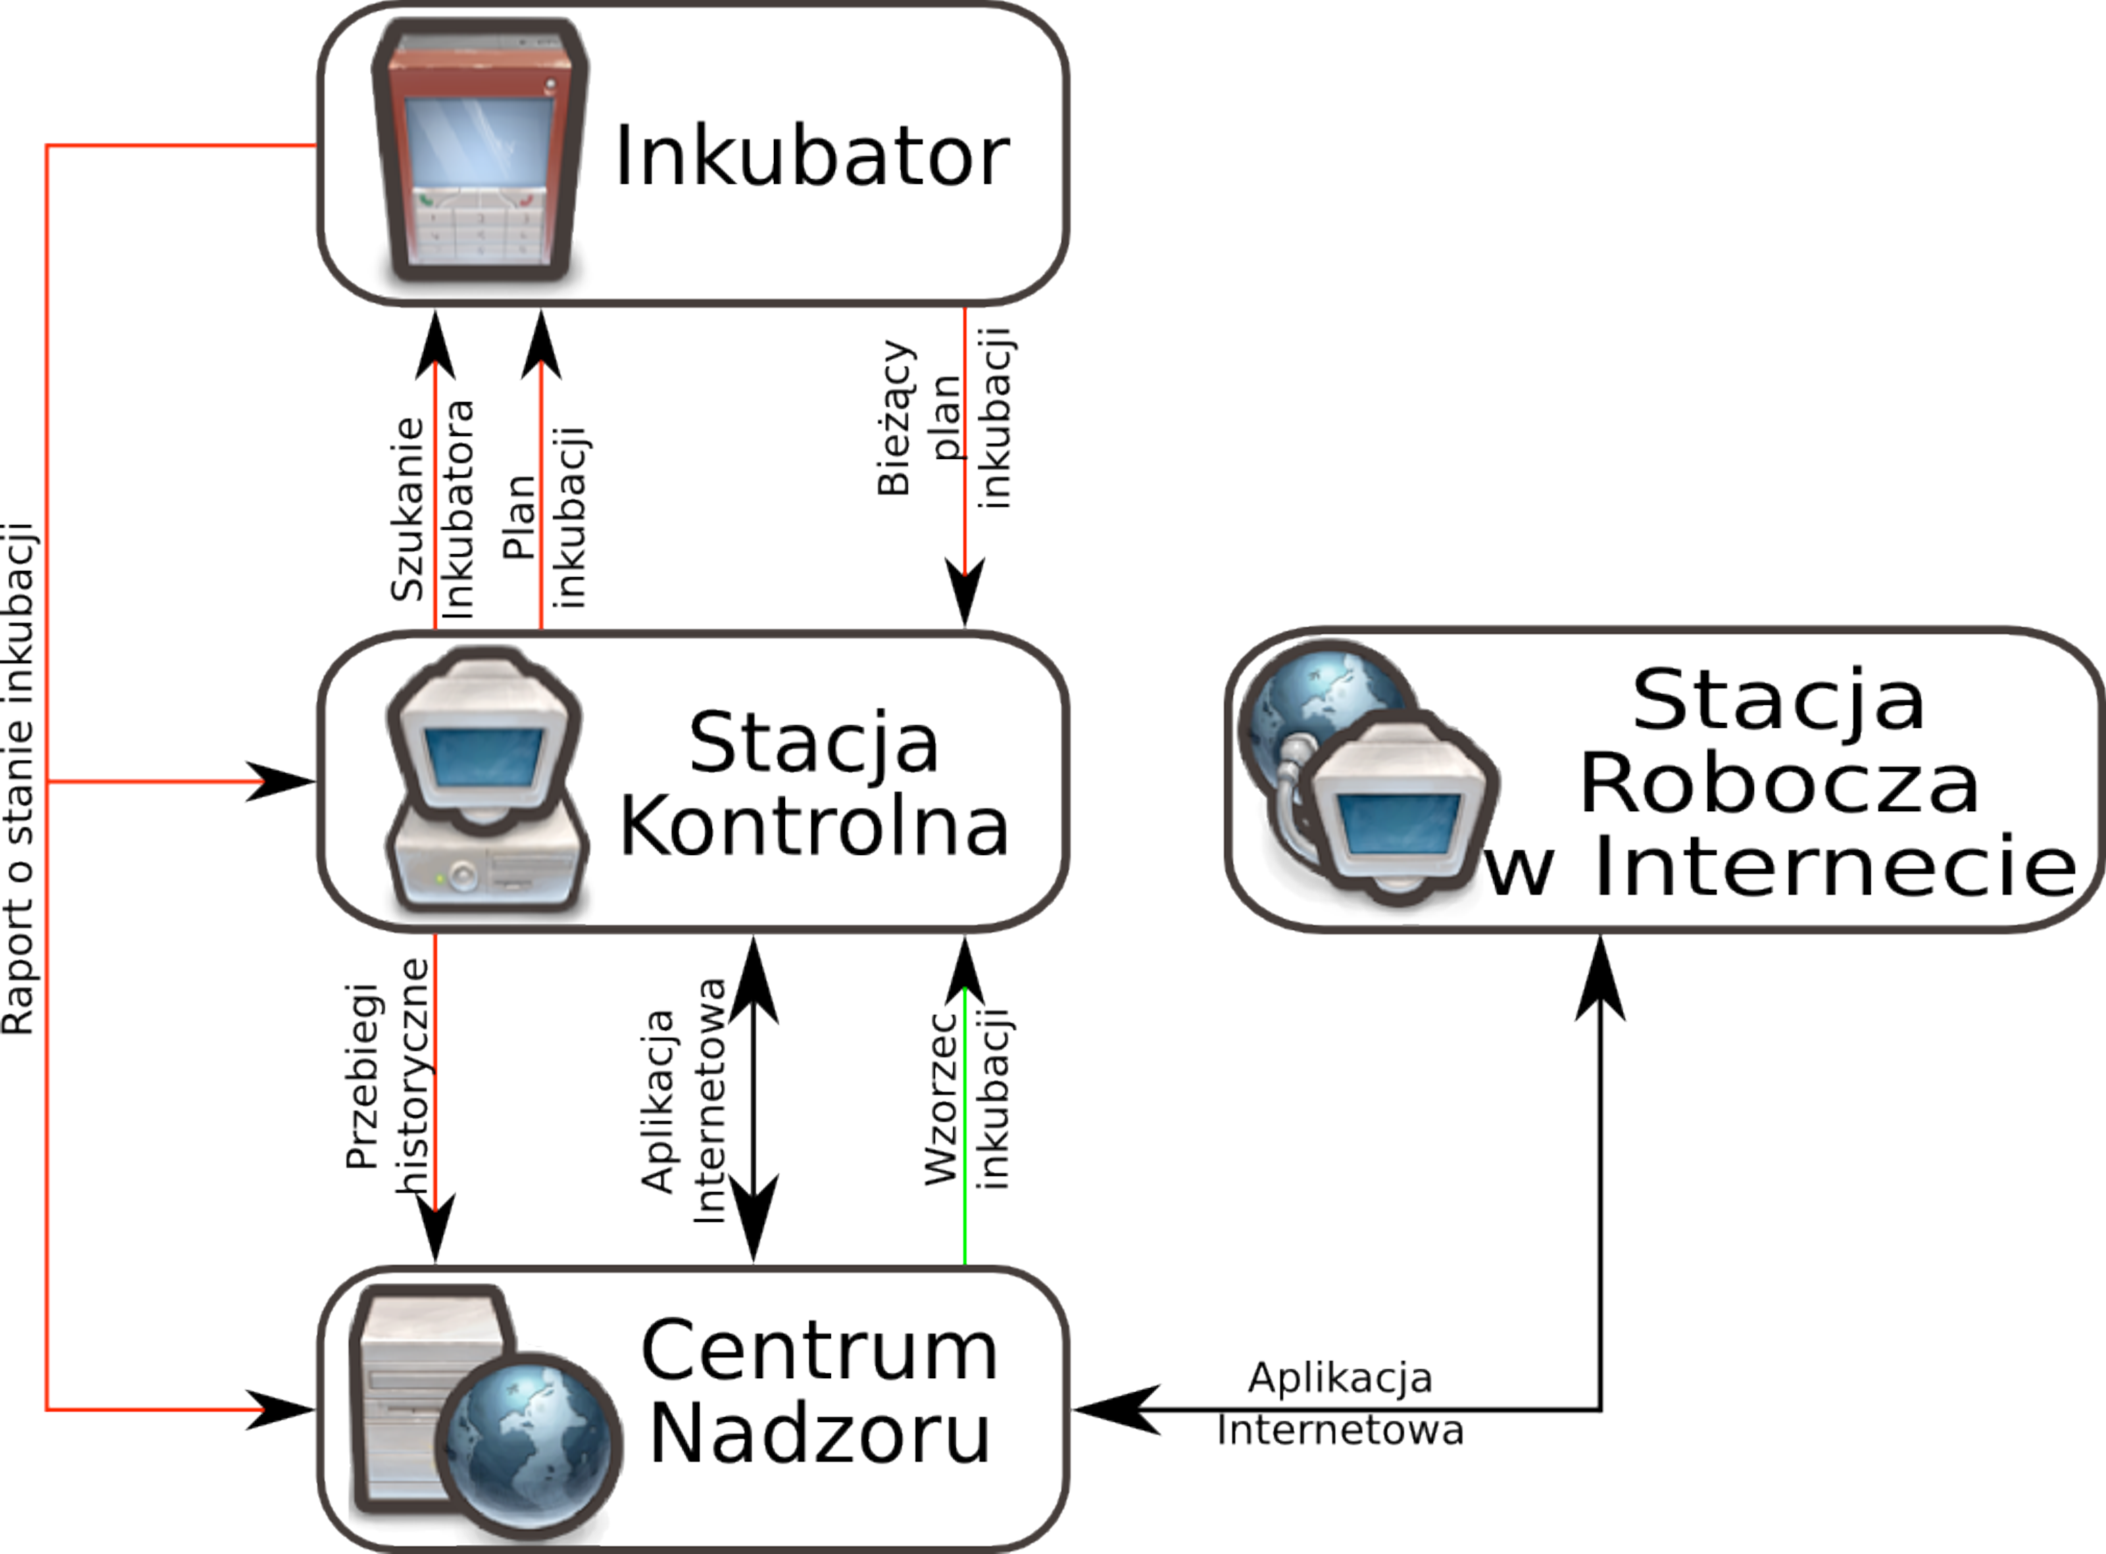
\includegraphics[width=.75\textwidth]{figures/Komunikacja}
\caption{Diagram komunikacji}\label{rys:Komunikacja}
\end{figure}

\subsection{Wykorzystane metody komunikacji}
\paragraph{Interfejs gniazd BSD}
System Thinkubator został zaimplementowany przy użyciu różnych języków
programowania (C, C\#, Phyton) oraz na różnych systemach operacyjnych (Gentoo
Linux, Windows XP), dlatego pożądany był sprawdzony interfejs komunikacji
sieciowej wspierany przez wszystkie powyższe technologie. Interfejs gniazd
został wykorzystany przy komunikacji na drodze Inkubator $\leftrightarrow$ Stacja Kontrolna,
Inkubator $\rightarrow$ Centrum Nadzoru oraz Stacja Kontrolna $\leftrightarrow$ Centrum Nadzoru.

W~każdej aplikacji uruchomiony jest osobny wątek odpowiedzialny za
odbieranie połączeń przychodzących. Wątek taki otwiera gniazdo na odpowiednim
porcie i~nasłuchuje na połączenia. W~momencie nawiązania połączenia wątek
nasłuchujący uruchamia kolejny wątek do obsługi połączenia, po czym powraca do
nasłuchiwania na nowe połączenia. Dzięki temu jakikolwiek błąd komunikacji nie
jest w~stanie zawiesić głównego wątku oczekującego na połączenia. Wykorzystane
porty to:
\begin{itemize}
	\item w~Inkubatorze port UDP BROADCAST\_PORT -- nasłuchiwanie na komunikat
		rozgłoszeniowy wysyłany przez Stację Kontrolną,
	\item w~Inkubatorze port TCP SCHEDULE\_PORT -- służący do odbierania ze Stacji
		Kontrolnej poleceń dotyczących pobrania/wysłania planu inkubacji, 
	\item w~Stacji Kontrolnej port TCP STATE\_REPORT\_PORT -- odbiór raportów
	z~inkubatora,
	\item w~Centrum Nadzoru port TCP STATE\_REPORT\_PORT -- odbiór raportów
	z~inkubatora lub Stacji Kontrolnej.
\end{itemize}

W~celu ujednolicenia protokołu komunikacji wszystkie pakiety przesyłane tą drogą
są zamknięte w~jedną z~dwóch struktur: struktura sterująca i~struktura danych.
Każdy akt komunikacji rozpoczyna się od przesłania jednej struktury sterującej
z~informacją o~typie rozkazu/komunikacji, który określa dalszy przebieg
komunikacji. Struktura danych służy do przesyłania raportów z~inkubatora,
historycznych przebiegów inkubacji oraz planów inkubacji. Definicja struktur
została przedstawiona w tabeli \ref{tab:Struktury}.
\begin{table}[t]
	\centering
	\begin{tabular}{m{7cm}|m{7cm}}
		\textbf{Control Structure:} &~\textbf{Data Structure:} \\
		& \verb+struct point_t {+ \\
		\verb+struct message_t {+ &~\verb+ int timestamp;+ \\
		\verb+ int deviceID;+ &~\verb+ int process_phase;+ \\
		\verb+ int processID;+ &~\verb+ double temperature;+ \\
		\verb+ int type;+ &~\verb+ double humidity;+ \\
		\verb+ int from_time;+ &~\verb+ int rolling;+ \\
		\verb+ int to_time;+ &~\verb+ double scheduled_temperature;+ \\
		\verb+ int amount;+ &~\verb+ double scheduled_humidity;+ \\
		\verb+}+ &~\verb+ int scheduled_rolling;+ \\
		& \verb+}+ \\
	\end{tabular}
	\caption{Definicja struktur komunikacyjnych}
	\label{tab:Struktury}
\end{table}

Ogólnie jednorazowa komunikacja odbywa się według algorytmu:
\begin{verbatim}
send( message_t header );
for i:=1 to header.amount do 
 send( point_t data );\end{verbatim}

\paragraph{Częściowe XML-RPC}
Stacja Kontrolna stosuje żądanie 
HTTP-GET do przesłania parametrów wywołania lub HTTP-POST do wysyłania danych
, zaś Centrum Nadzoru używa języka XML do
zakodowania wyników wywołania oraz HTTP jako protokołu transportowego. XML-RPC
jest również niezależny od platformy sprzętowej i~języka programowania. 
Odpowiedź XML dostosowana jest do formatu w~jakim Stacja Kontrolna przechowuje swoje dane. 
Technologia ta została wykorzystana gdy:
\begin{itemize}
\item Stacja Kontrolna pobiera z~Centrum Nadzoru wzorce inkubacji, 
\item Stacja Kontrolna pobiera z~Centrum Nadzoru informacje o~znanych gatunkach,
\item Stacja Kontrolna wysyła do Centrum Nadzoru informację o~rozpoczęciu inkubacji,
\item Stacja Kontrolna wysyła do Centrum Nadzoru informację o~zakończeniu inkubacji,
\end{itemize}

\section{Stacja kontrolna}
Aplikacja działająca na Stacji Kontrolnej została napisana w~środowisku
Visual Studio .NET 2005 \cite{MSDN}, w~języku programowania C\#. Ponadto program
wykorzystuje zewnętrzną bibliotekę graficzną \akronim{CSGL} (\english{C\#
Graphics Library}). Stacja Kontrolna spełnia dwa główne
zdania: monitorowanie oraz programowanie inkubatorów.

Monitorowanie realizowane jest poprzez mechanizm wysyłania z~inkubatorów
raportów z~wartościami sterowanych parametrów inkubacji. W~równych odstępach czasu Stacja Kontrolna rejestruje pakiet
danych od inkubatora z~informacją o~zaplanowanych i~aktualnych warunkach
panujących w~inkubatorze. Na tej podstawie Stacja Kontrolna wyświetla na ekranie aktualny stan
wszystkich zarejestrowanych inkubatorów oraz ogólny przebieg temperatury
i~wilgotności w~ciągu ostatniej doby. Po wybraniu dowolnego inkubatora Stacja Kontrolna
wyświetla szczegółowy przebieg sterowanych parametrów, obejmujący pełny okres
inkubacji. Dzięki wykorzystaniu biblioteki \emph{CSGL} możliwa jest płynna nawigacja
po wykresie, zbliżenie na dowolny okres czasu lub dowolne wartości temperatury
i~wilgotności.

Funkcjonalność programowania inkubatora pozwala na precyzyjny dobór nastawu inkubatora
w~bardzo prosty sposób. Przy tworzeniu nowego planu inkubacji ornitolog wybiera
inkubowane gatunki, zaś Stacja Kontrolna dobiera do nich wzorce inkubacji i~wizualizuje je na
ekranie. Półprzezroczyste wzorce inkubacji dla różnych gatunków są nakładane na siebie,
dzięki czemu widoczne są rozbieżności w~pożądanych przebiegach
temperatury i~wilgotności. Pozwala to na podjęcie decyzji o~dopuszczeniu różnych
gatunków do wspólnej inkubacji i~dobór optymalnego planu inkubacji. Utworzony
plan inkubacji może zostać zapisany na dysku lub przesłany do wybranego
inkubatora. Stacja Kontrolna pozwala też na pobranie z~inkubatora jego aktualnego planu
i~wprowadzenie w~nim dowolnych zmian.

\begin{figure}[b] 
\centering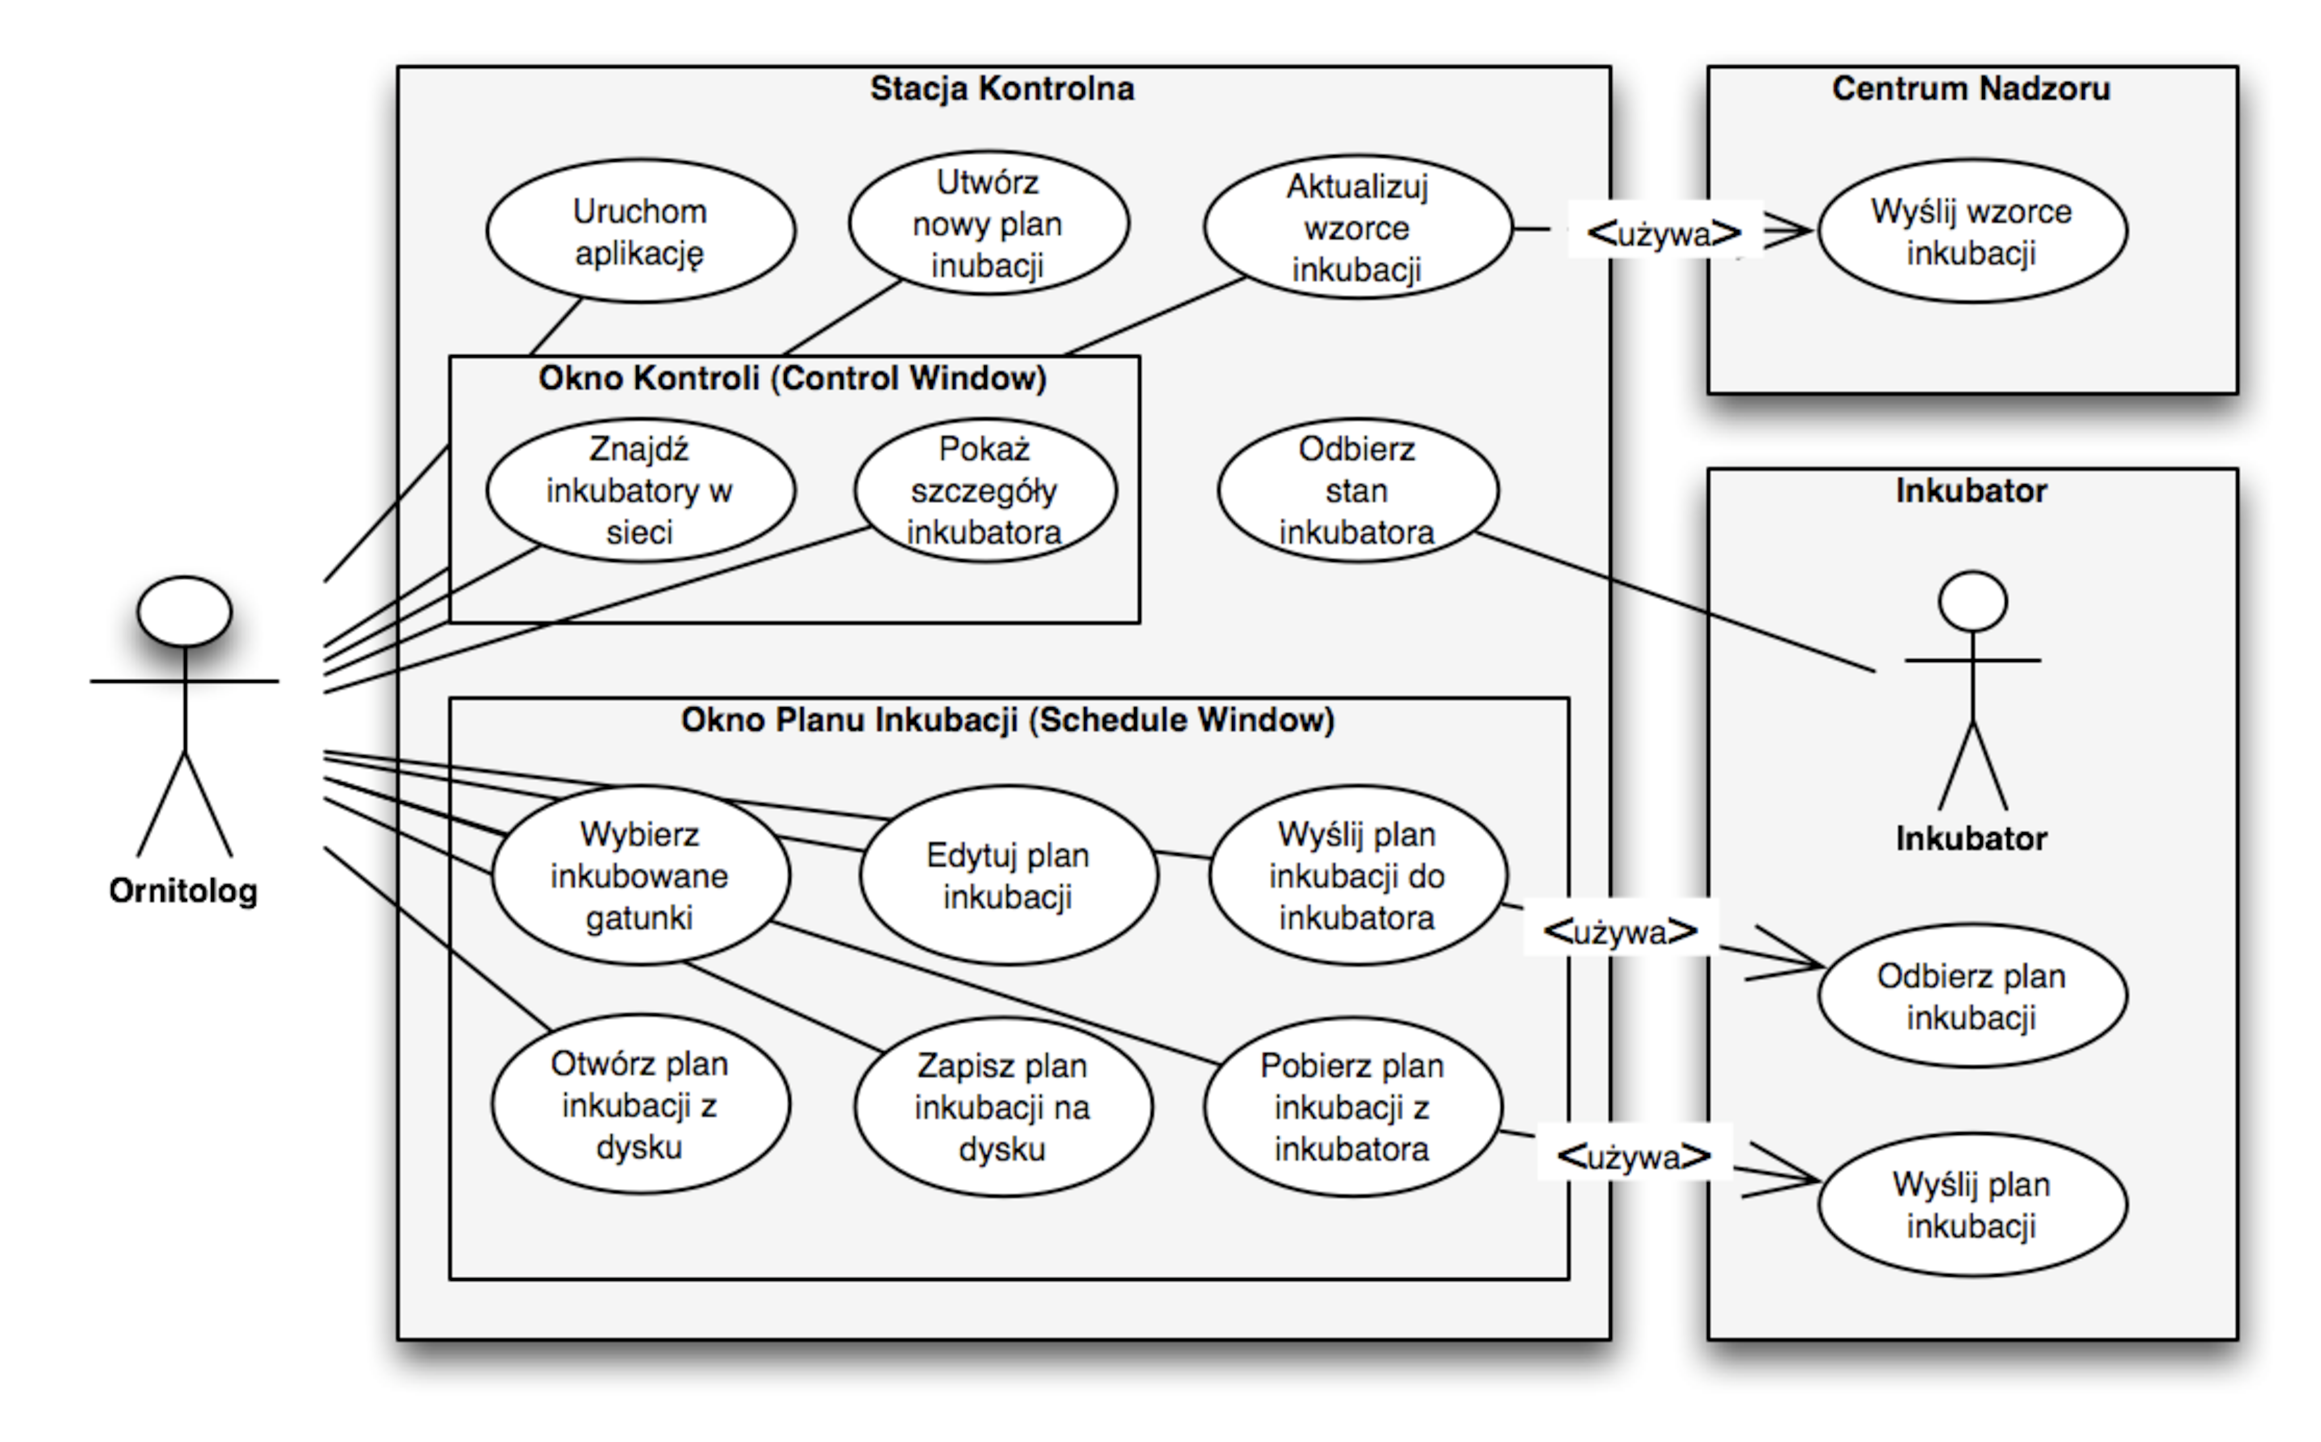
\includegraphics[width=\textwidth]{figures/CSUseCase}
\caption{Diagram przypadków użycia stacji kontrolnej}\label{rys:CSUseCase}
\end{figure}

\subsection{Przypadki użycia}
Podczas projektowania aplikacji przeprowadzono konsultacje z~użytkownikami końcowymi
i~przeanalizowano wymaganą oraz pożądaną funkcjonalność programu.
W rezultacie wyznaczono 12 przypadków użycia, które ilustruje rysunek \ref{rys:CSUseCase}. 
\pagebreak

\noindent Poszczególne przypadki użycia zdefiniowane są następująco:\\
Aktorzy:
\begin{enumerate}
	\item Ornitolog -- osoba przeprowadzająca/nadzorująca inkubację,
	\item Inkubator -- aplikacja inkubatora,
	\item Stacja Kontrolna -- opisywany system,
	\item Centrum Nadzoru -- zdalny serwer.
\end{enumerate}

\begin{itemize}
	\item[\textbf{UC1}] Uruchomienie aplikacji.
		\begin{enumerate}
			\item Ornitolog uruchamia aplikację Stacji Kontrolnej.
			\item Stacja Kontrolna uruchamia wątek oczekujący na przychodzące połączenia z~sieci.
			\item Stacja Kontrolna wysyła w~sieć lokalną wiadomość rozgłoszeniową z~własnym adresem IP, celem poinformowania o~nim Inkubatorów.
			\item Stacja Kontrolna oczekuje klika sekund na odpowiedź Inkubatorów.
			\item Stacja Kontrolna rejestruje znalezione Inkubatory.
			\item Stacja Kontrolna wyświetla główne okno aplikacji, Control Window.
		\end{enumerate}

	\item[\textbf{UC2}] Znajdź inkubatory w~sieci.
		\begin{enumerate}
			\item Ornitolog wybiera z~menu opcję ,,Find incubators''.
			\item Stacja Kontrolna wysyła w~sieć lokalną wiadomość rozgłoszeniową z~własnym adresem IP, celem poinformowania o~nim Inkubatorów.
			\item Stacja Kontrolna oczekuje klika sekund na odpowiedź Inkubatorów.
			\item Stacja Kontrolna rejestruje znalezione Inkubatory.
		\end{enumerate}


	\item[\textbf{UC3}] Pokaż szczegóły inkubatora.
		\begin{enumerate}
			\item Ornitolog wybiera jeden z~inkubatorów widocznych w~głównym oknie aplikacji.
			\item Stacja Kontrolna wyświetla szczegółowy wykres wybranego inkubatora.
			\item Ornitolog dowolnie nawiguje po wykresie, manipulując osiami czasu, temperatury i~wilgotności.
		\end{enumerate}

	\item[\textbf{UC4}] Utwórz nowy plan inkubacji.
		\begin{enumerate}
			\item Ornitolog wybiera opcję ,,Schedule Tool'' z~menu aplikacji.
			\item Stacja Kontrolna wyświetla okno do tworzenia planu inkubacji (Schedule Window).
		\end{enumerate}

	\item[\textbf{UC5}] Edytuj listę gatunków.
		\begin{enumerate}
			\item Ornitolog wybiera z~menu opcję ,,Birds''.
			\item Stacja Kontrolna wyświetla dialog wyboru gatunków.
			\item Ornitolog wybiera inkubowane gatunki i~zatwierdza wybór.
			\item Stacja Kontrolna aktualizuje wzorzec inkubacji w~oknie planu inkubacji.
		\end{enumerate}

	\item[\textbf{UC6}] Zapisz plan inkubacji na dysku.
		\begin{enumerate}
			\item Ornitolog wybiera z~menu opcję zapisania planu inkubacji (,,Save'').
			\item Stacja Kontrolna wyświetla dialog wyboru pliku.
			\item Ornitolog wybiera plik do zapisu planu inkubacji.
			\item Stacja Kontrolna zapisuje plan inkubacji.
		\end{enumerate}

	\item[\textbf{UC7}] Wczytaj plan inkubacji z~dysku.
		\begin{enumerate}
			\item Ornitolog wybiera z~menu opcję wczytania planu inkubacji (,,Open'').
			\item Stacja Kontrolna wyświetla dialog wyboru pliku.
			\item Ornitolog wybiera plik do wczytania planu inkubacji.
			\item Stacja Kontrolna wczytuje plan inkubacji.
		\end{enumerate}

	\item[\textbf{UC8}] Edytuj plan inkubacji.
		\begin{enumerate}
			\item Ornitolog wybiera z~paska narzędzi edytowaną funkcję (temperatura, wilgotność lub rolowanie).
			\item Ornitolog nanosi wartości pożądanej funkcji na wykres.
		\end{enumerate}

	\item[\textbf{UC9}] Wyślij plan inkubacji do inkubatora.
		\begin{enumerate}
			\item Ornitolog wybiera z~menu opcję wysłania planu inkubacji do Inkubatora (,,Send schedule'').
			\item Stacja Kontrolna wyświetla dialog wyboru inkubatora.
			\item Ornitolog wybiera inkubator.
			\item Stacja Kontrolna wysyła do Inkubatora informację o~zmianie planu inkubacji.
			\item Inkubator akceptuje zmianę.
			\item Stacja Kontrolna wysyła plan inkubacji.
			\item Inkubator odbiera plan inkubacji.
			\item Stacja Kontrolna informuje Ornitologa o~poprawnie wykonanej operacji.
		\end{enumerate}

	\item[\textbf{UC10}] Pobierz plan inkubacji z~inkubatora.
		\begin{enumerate}
			\item Ornitolog wybiera z~menu opcję pobrania planu inkubacji do inkubatora (,,Retrieve schedule'').
			\item Stacja Kontrolna wyświetla dialog wyboru inkubatora.
			\item Ornitolog wybiera inkubator.
			\item Stacja Kontrolna wysyła do Inkubatora żądanie planu inkubacji.
			\item Inkubator wysyła plan inkubacji.
			\item Stacja Kontrolna odbiera plan inkubacji.
			\item Stacja Kontrolna wyświetla pobrany plan inkubacji.
			\item Stacja Kontrolna informuje Ornitologa o~poprawnie wykonanej operacji.
		\end{enumerate}

	\item[\textbf{UC11}] Aktualizuj wzorce inkubacji.
		\begin{enumerate}
			\item Ornitolog wybiera z~menu opcję uaktualnienia wzorców.
			\item Stacja Kontrolna pobiera wzorce inkubacji z~Centrum Nadzoru poprzez HTTP.
			\item Stacja Kontrolna informuje Ornitologa o~poprawnie wykonanej operacji.
		\end{enumerate}

	\item[\textbf{UC12}] Odbierz stan inkubatora.
		\begin{enumerate}
			\item Inkubator wysyła do Stacji Kontrolnej pakiet danych pomiarowych z~informacją o~warunkach panujących aktualnie w~komorze inkubacyjnej.
			\item Stacja Kontrolna odbiera pakiet danych.
			\item Jeśli inkubator nie był wcześniej wykryty, zostaje on zarejestrowany w~Stacji Kontrolnej.
			\item Stacja Kontrolna dodaje otrzymany pakiet danych do historii inkubacji danego Inkubatora.
			\item Stacja Kontrolna zapisuje historię inkubacji danego Inkubatora na dysku.
		\end{enumerate}
\end{itemize}


\subsection{Architektura aplikacji}
Architektura aplikacji Stacji Kontrolnej zgodna jest z~podziałem funkcjonalności na monitorowanie i~programowanie inkubatorów.
Funkcje te zostały zaimplementowane w~dwóch klasach dziedziczących
z~klasy \emph{Form}, o~nazwie odpowiednio \emph{ControlWindow} i~\emph{ScheduleWindow}. Okna te są zintegrowane
w~głównym oknie aplikacji (\emph{ControlStation}). Algorytmy komunikacji sieciowej implementuje statyczna klasa
\emph{Listener}. Klasa ta zawiera również kolekcję obiektów klasy \emph{Icubator}, które reprezentują znajdujące się w~sieci Inkubatory.
Szczegółowy diagram klas przedstawiony jest na rysunku~\ref{rys:CSClass}.

\begin{figure}[h] 
\centering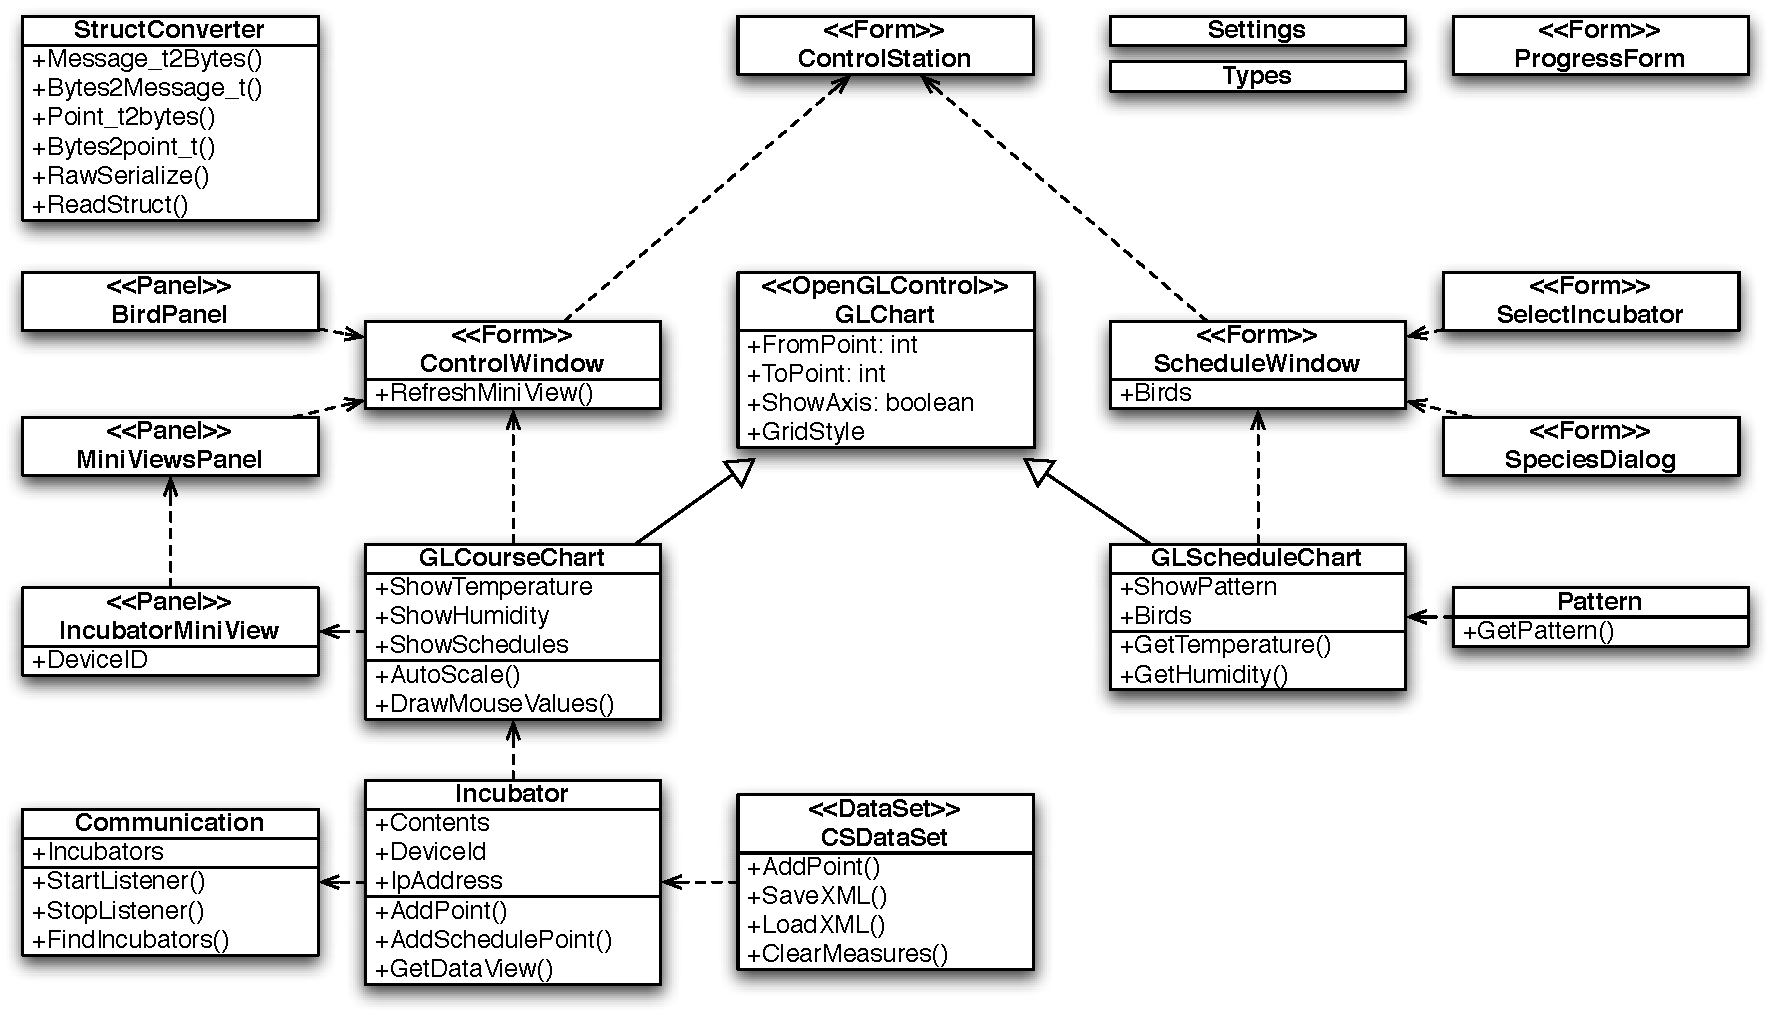
\includegraphics[width=\textwidth]{figures/CSClass}
\caption{Diagram klas aplikacji działającej na Stacji Kontrolnej}\label{rys:CSClass}
\end{figure}

\noindent Opis klas tworzących aplikację Stacji Kontrolnej:
\begin{itemize}
	\item ControlStation -- główne okno aplikacji,
	\item ControlWindow -- okno kontrolne, zawsze otwarte w~głównym oknie aplikacji, zawiera widok listy inkubatorów i~podgląd wybranego inkubatora,
	\item GLChart -- kontrolka dziedzicząca z~klasy \emph{OpenGLControl} umożliwiająca renderowanie wykresów przy użyciu biblioteki \emph{CSGL},
	\item GLCourseChart -- kontrolka dziedzicząca z~klasy \emph{GLChart}, dostosowana do renderowania przebiegów temperatury i~wilgotności,
	\item MiniViewsPanel -- kontrolka, na której wyświetlana jest lista kontrolek typu \emph{IncubatorMiniView},
	\item IncubatorMiniView -- kontrolka, na której wyświetlana jest informacja o~warunkach panujących w~inkubatorze oraz wykres temperatury i~wilgotności z~ostatniej doby,
	\item BirdPanel -- kontrolka, na której wyświetlana jest lista gatunków w~wybranym inkubatorze,
	\item ScheduleWindow -- okno do programowania inkubatora,
	\item ScheduleChart -- kontrolka dziedzicząca z~klasy \emph{GLChart}, dostosowana do nanoszenia planu inkubacji,
	\item Pattern -- klasa reprezentująca wzorce inkubacji,
	\item SpeciesDialog -- dialog wyboru inkubowanych gatunków,
	\item SelectIncubator -- dialog wyboru inkubatora, służy do wysyłania i~pobieranie planu inkubacji z~inkubatora,
	\item Incubator -- klasa reprezentująca inkubator, zawiera informacje o~zawartości inkubatora i~bieżącym procesie inkubacji,
	\item CSDataSet -- zbiór danych pomiarowych z~przebiegu inkubacji,
	\item Communication -- statyczna klasa odpowiedzialna za komunikację sieciową, zawiera inkubatory zarejestrowane w~systemie,
	\item ProgressForm -- okno z~paskiem postępu wyświetlanym w~trakcie szukania inkubatorów,
	\item Settings -- ustawienia aplikacji zapamiętywane w~rejestrze systemowym,
	\item Types -- klasa zawierająca definicję typów strukturalnych i~wyliczeniowych,
	\item TimeConverter -- statyczna klasa udostępniająca metody konwersji czasu między
		formatami stosowanymi w~C\# i~C,
	\item StructConverter -- statyczna klasa udostępniająca metody konwersji struktur do strumienia bajtów wysyłanych przez sieć.
\end{itemize}

\section{Centrum nadzoru}
%[[Tak jak można by powiedzieć że inkubatory to mięśnie naszego systemu, a~stacje kontroli -- nerwy, to serwer jest mózgiem naszego systemu.]]
Centrum Nadzoru jest dopełnieniem systemu Thinkubator, które choć nie jest niezbędne
do prowadzenia inkubacji, to daje niespotykane dotychczas możliwości. Jest ono odpowiedzialne za:
\begin{itemize}
	\item gromadzenie danych z~przebiegu inkubacji (zaprogramowane i~rzeczywiste wartości sterowanych parametrów),
	\item monitorowanie bieżącego stanu inkubatorów,
	\item wizualizacja dotychczasowego przebiegu każdej inkubacji,
	\item informowanie o~stanie wiedzy na temat gatunków,
	\item analiza danych celem tworzenia wzorców,
	\item alarmowanie o~błędach,
	\item kontrola dostępu użytkowników do poszczególnych funkcji systemu,
	\item zarządzanie kontami użytkowników.
\end{itemize}
W tej chwili nie ma ono pełnej oczekiwanej funkcjonalności gdyż analiza danych w~takim systemie to bardzo złożony problem wymagający długotrwałych badań zarówno na poziomie informatyki jak i~biologii. Obecna implementacja jest podstawą do dalszego rozwoju.

\subsection{Technologia}
Ze względu na krótki czas rozwoju i~duże wymagania dla Centrum Nadzoru, do
implementacji postanowiono użyć środowiska progamistycznego TurboGears
\cite{TurboGears} napisanego w~języku Python. Jest to jedno z~najnowszych
z~narzędzi służących do rozwoju internetowych aplikacji w~architekturze
\akronim{MVC} (\english{Model, View, Controller}). Wnioski z~testów
przeprowadzonych przez niezależnego eksperta sugerują, że można około 9~razy
szybciej rozwijać aplikacje internetowe w~TG niż przy użyciu \akronim{J2EE}
(\english{Java 2~Enterprise Edition}), zakładając że wykorzystano
\emph{Hibernate} jako warstwę trwałości. Przy zastosowaniu \akronim{EJB}
(\english{Enterprise JavaBeans}) przewaga TG rośnie jeszcze bardziej, oczywiście
w~teście założono nierozróżnialność jakościową (funkcjonalność, wydajność itd.)
aplikacji. Oprócz tego TG udostępnia aplikacje do zarządzania bazą danych oraz
wspiera wykorzystanie \akronim{AJAX} (\english{Asynchronous JavaScript And
XML}), co będzie miało znaczenie również przy rozbudowywaniu naszego systemu.
TG aktywnie korzysta z~infrastruktury setuptools \cite{setuptools} -- dzięki
czemu można korzystać z~różnego rodzaju modułów przygotowanych i~udostępnianych
przez użytkowników systemu np.: generator wykresów PlotKit \cite{PlotKit}. Przy
tworzeniu bazy danych skorzystano z mapera obiektowo relacyjnego
\emph{SQLObject}. Jako bazę danych wykorzystano MySQL ze względu na jego
szybkość, łatwość obsługi i~dostępność dokumentacji. Warstwa trwałości jest
niezależna od bazy danych więc w~razie potrzeby można bazę danych zmienić. 

\subsection{Baza danych}
\begin{figure}[t]
\centering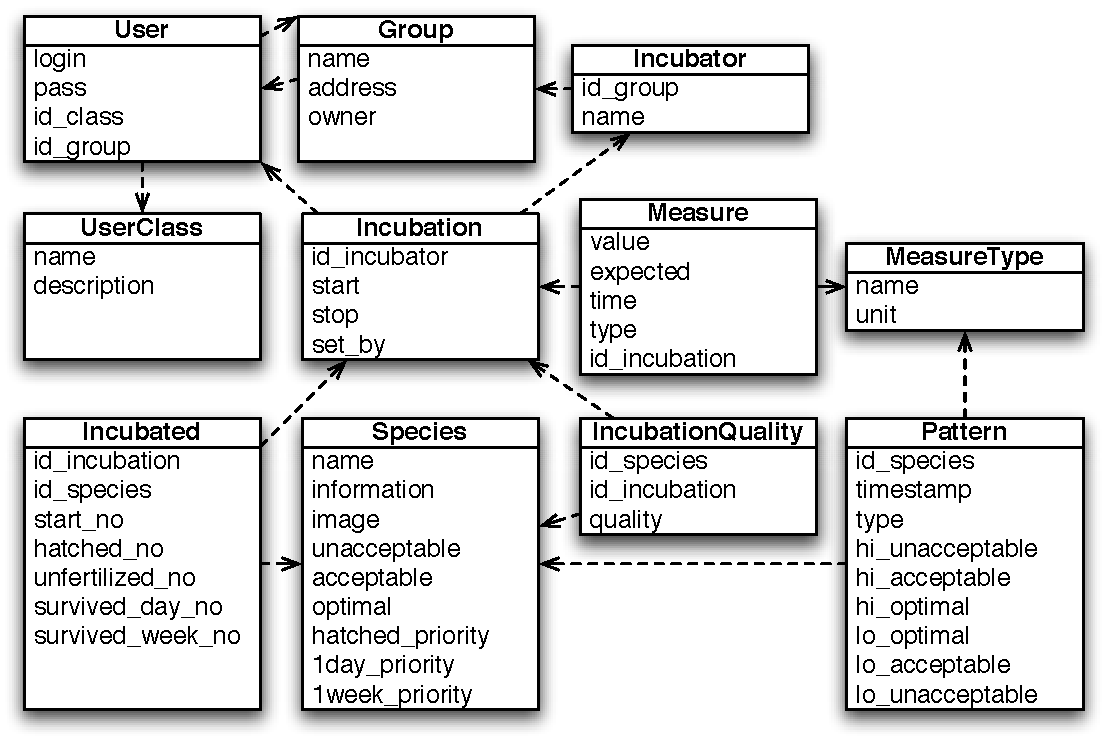
\includegraphics[width=\textwidth]{figures/SCCDataBase}
\caption{Schemat bazy danych centrum nadzoru}\label{rys:SCCDataBase}
\end{figure}

Relacyjny schemat tabel bazy danych przedstawiono na rysunku
\ref{rys:SCCDataBase}. Poniżej przedstawiony jest krótki opis tabel znajdujących
się na nim:
\begin{itemize}
	\item \textbf{Group} -- opisuje grupy użytkowników. Najczęściej
		występującą grupą będą pracownicy jakiejś instytucji mający dostęp do
		określonej puli Inkubatorów. Grupa ma właściciela (pole owner), może on
		edytować użytkowników grupy. 
	\item \textbf{User} -- opisuje Użytkowników systemu. Użytkownik może
		należeć do różnych klas z~tabeli UserClass.
	\item \textbf{UserClass} -- krotki w~tej tabeli odpowiadają klasom użytkowników.
		Dla każdej klasy użytkowników zdefiniowane są w~systemie pewne prawa
		dostępu. 
	\item \textbf{Incubator} -- opisuje Inkubatory. Inkubator należy do
		grupy użytkowników. Użytkownik może go opisać, aby było mu łatwo rozróżnić
		Inkubatory.
	\item \textbf{Measure} -- opisuje pomiary z~czujników w~Inkubatorze.
		Pomiar dotyczy inkubacji oraz ma typ z~tabeli MeasureType. Każdy pomiar jest
		również umiejscowiony w~czasie.
	\item \textbf{MeasureType} -- zawiera typy pomiarów (np. temperatura,
		wilgotność).
	\item \textbf{Incubation} -- opisuje inkubację: na którym inkubatorze
		jest przeprowadzona, w~jakim czasie i~kto ją zainicjował. 
	\item \textbf{Inlubated} -- opisuje wynik inkubacji dla danego gatunku.
		System zapamiętuje ilość jaj, ilość wyklutych piskląt oraz ilość
		piskląt, które przeżyły 24 godziny oraz pierwszy tydzień. Dla zoologów są to
		bardzo ważne dane gdyż większość piskląt umiera podczas pierwszego tygodnia po wykluciu.
		Może się więc okazać, że mimo iż pewne inkubacje są nierozróżnialne pod
		względem klujności, to przeżywalność w~dłuższym czasie się zmienia. 
	\item \textbf{Species} -- zawiera podstawowe dane o~gatunkach.
	\item \textbf{DataAnalisys} -- zawiera dane o~jakości inkubacji (pole
		,,parameters''). Są one generowane w~oparciu o~wartości pomiarów dla danej
		inkubacji oraz jej wynik. Jakość inkubacji jest wagą w~oparciu o~którą
		generowany jest wzorzec inkubacji dla danego gatunku. 
	\item \textbf{Pattern} -- przechowuje wzorzec inkubacji dla
		danego gatunku. Opisuje on chwile w~czasie i~przyporządkowuje im nastawy
		które są pożądane, dopuszczalne i~niedopuszczalne. Pole ,,type'' determinuje czy
		krotka opisuje wilgotność czy temperaturę. 
\end{itemize}

\subsection{Implementacja}
W~tym podrozdziale zostały opisane szczegóły implementacj Centrum Nadzoru.
Wynikają one z architektury TurboGears. Cała aplikacja składa się z~obiektów
czterech rodzajów:
\begin{itemize}
	\item \textbf{Wzorców} -- są to klasy wygenerowane z~języka wzorców Kid
		\cite{KID}. Wzorce reprezentują warstwę prezentacji aplikacji. Język Kid
		opiera się o~XHTML. Przy jego pomocy projektowane były komponenty Wizualne.
		Przed uruchomieniem aplikacji kontroler TurboGears zamienia wzorce na
		obiekty, które są wywoływane przez Kontrolery. 
	\item \textbf{Komponentów} -- są to klasy specyficzne dla TurboGears.
		Komponenty są klasami, które dodają do Wzorców pewną funkcjonalność. Wzorzec
		tylko wygląda, a~komponent jeszcze posiada pewną funkcjonalność. Komponent
		może się składać z~wielu innych komponentów (np. formularz) oraz z~wielu
		wzorców. Komponenty korzystają transparentnie z~biblioteki MochiKit,
		ułatwiając implementację komponentów korzystających z~technologii
		\akronim{AJAX}.
	\item \textbf{Klasy modelu} -- implementują one klasy mapera obiektowo
		relacyjnego \emph{SQLObject}. Klasy modelu reprezentują krotki w~bazie
		danych. Klasy modelu są typów zgodnych z~typami tabel bazy danych. Baza
		danych została utworzona w~oparciu implementację klas modelu.
	\item \textbf{Kontrolerów} -- implementują one elementy serwera Cherrypy.
		Kontrolery łączą ze sobą wszystkie pozostałe klasy. One wykonują zapytania
		w~oparciu o~dane wejściowe przy pomocy klas modelu,obrabiają je i~wywołują
		wzorce lub komponenty z~odpowiednimi parametrami.
\end{itemize}
W następnej części dokumnetu bardziej szczegółowo opisano najważniejsze części
aplikacji.

\paragraph{Kontrolery:}
\begin{itemize}
\item \textbf{Index} -- domyślny kontrtoler odpowiada za wygląd i~strukturę
	dokumentu.
\item \textbf{Info} -- jest on implementacją prostego systemu zarządzania
	treścią CMS, zawiera ogólne informacje o~projekcie.
\item \textbf{Incubators} -- implementuje system pozwalający śledzić stan
	inkubatorów,
\item \textbf{Incubations} -- ten kontroler pozwala śledzić stan inkubacji
	(zmienne procesowe inkubatora). Pozwala edytować ilość jaj poszczególnych
	gatunków oraz wyniki inkubacji. 
\item \textbf{Species} -- ten kontroler jest odpowiedzialny za wyświetlanie
	stanu wiedzy systemu o~poszczególnych gatunkach (np. ilość inkubacji, średnia
	klujność oraz wzorce inkubacji).
\item \textbf{Plotter} -- ten kontroler jest odpowiedzialny za generowanie
	odpowiednich wykresów.
\item \textbf{XML-RPC} zajmuje się odpowiadaniem na zapytania Stacji Kontrolnej.
	W momencie gdy Stacja kontrolna potwierdzi zakończenie inkubacji, uruchamia on
	także generator wzorców.
\item \textbf{Catwalk} jest komponentem służącym bezpośrednio do przeglądania bazy danych. W~tej chwili funkcjonalność administracyjna jest bardzo ograniczona. Zakłada się, że jest jeden administrator, który bezpośrednio edytuje zawartość bazy danych przy pomocy tego komponentu.
\end{itemize}

\paragraph{Generowanie wzorców.}
W tej chwili do dyspozycji jest prosty algorytm generujący wzorce, oparty
o~linearyzację wag inkubacji i~ich pomiarów. Dla każdej inkubacji liczona jest
jej waga ($W$), równoważna klujności danego gatunku w~danej inkubacji. Jest ona
liczona w~oparciu o~stosunek ilości piskląt, które się wykluły ($p_w$), piskląt,
które przeżyły 24 godziny ($p_{24}$) oraz piskląt, które przeżyły tydzień
($p_t$) oraz wag dla tych ilości ustalonych dla danego gatunku -- odpowiednio:
$w_w$, $w_{24}$ i~$w_t$, do ilości zalężonych jaj ($j_z$) pomnożonych przez sumę
wag. Końcowy wzór przedstawiono w równaniu \ref{eq:wagi}.

\begin{equation}
	\label{eq:wagi}
	W =~\frac{p_w \cdot w_w +~p_{24} \cdot w_{24} +~p_t \cdot w_t }{(w_w +~w_{24} +~w_t) \cdot j_z} 
\end{equation}

W każdym punkcie pomiarowym generowana jest funkcja wagi $W$ od pomiaru $m$ -- $W(m)$. 
Funkcja $W(m)$ przyporządkowuje każdemu pomiarowi m~w danej chwili wartość wagi inkubacji z~jakiej ten pomiar pochodzi ($W$).
Na tą przestrzeń ($W(m)$) rzutowane są wartości charakteryzujące wszystkie inkubacje danego gatunku.
Tak więc dla danej inkubacji trwającej 2~tygodnie, dla której pomiary zbierane są co 5~minut otrzymujemy
$2 \cdot 7~\cdot 24 \cdot 12 \approx 4000$ przyporządkowań wartości $W$ do pomiaru $m$.

Wartości maksymalne tej funkcji stają się podstawą podziału na kategorie
w~oparciu o~klujność danego gatunku. Skrajne temperatury, których wartość
odpowiada wartości odcięcia klas dla danego gatunku stają się odpowiednio
najniższą i~najwyższą akceptowaną temperaturą w~danej klasie. W~tej chwili
rozróżniamy 3~klasy: optymalna, akceptowalna i~nieakceptowalna.

\paragraph{Generowanie wykresów.}
Do generowania wykresów wykorzystano bibliotekę \emph{PlotKit} zaimplementowaną
w~języku JavaScript. Istnieje moduł \emph{TurboPlotKit}, który udostępnia
funkcjonalność tej biblioteki bezpośrednio w~środowisku TurboGears. Biblioteka
ta generuje pliki \akronim{SVG} (\english{Scalable Vector Graphic}) z~danych
wysłanych z~serwera. Przeglądarka internetowa renderuje te pliki do postaci
obrazów, które są wyświetlane użytkownikowi. Wykresy są generowane i~renderowane
na komputerze użytkownika. Dzięki temu obciążenie serwera jest minimalne --
pobiera on dane z~bazy danych i~zamieszcza je w~kodzie strony. Komputer klienta
obrabia je, a~następnie renderuje z~nich obraz. Badano również zastosowanie
biblioteki matplotlib, ale zrezygnowano z~jej wykorzystania ze względów
wydajnościowych, gdyż w~przypadku jej wykorzystania to Centrum Nadzoru
renderowało obraz, który użytkownik pobierał. Taki mechanizm utrudniał
dostosowanie wykresu do wymagań użytkownika oraz powodował duże obciążenie
procesora oraz łącza internetowego Centrum Nadzoru. 

\paragraph{Wydajność.}
Początkowo wykresy generowane były w~momencie przybycia nowych danych za
pośrednictwem gniazd \emph{BSD} (komunikacja z~Inkubatorem) albo \emph{XML-RPC}
(komunikacja ze Stacją Kontrolną) i~zapisywane do odpowiednich katalogów przy
pomocy biblioteki \emph{matplotlib}. Wygenerowane wykresy są formatu
\akronim{PNG} (\english{Portable Network Graphics}). Zdecydowano, aby wykresy
były generowane w~momencie przybycia danych, a~nie w~momencie nadejścia żądania
danego wykresu od użytkownika aplikacji internetowej.  Zaobserwowano, że wąskim
gardłem serwera jest generowanie wykresów stanu inkubacji co 5~minut, gdy
nadejdą nowe dane z~inkubatorów. Wszystkie inne wymagające mocy obliczeniowej
zdarzenia zachodzą bardzo rzadko (aktualizacja wzorców zachodzi na koniec
inkubacji która trwa 2-8~tygodni). Większą część interaktywnej aplikacji
internetowej można przechowywać w~pamięci operacyjnej (\emph{RAM cache}), a~jej
logika biznesowa nie obciąża zbytnio procesora.  Dlatego zastosowano bibliotekę
\emph{PlotKit}, która przenosi obciążenie związane z~generowaniem wykresu na
użytkownika, dzięki czemu odciąża Centrum Nadzoru z~najbardziej kosztownego
obliczeniowo zadania.

\paragraph{Testowanie.}
TG ma system wspierający automatyczne testowanie z~którego skorzystano przy
testach jednostkowych. Ponadto przeprowadzono interaktywne testy ,,czarnej
skrzynki'', w~których uczestniczyli członkowie zespołu.


